% Diagnosing and Repairing Minimal-Data Activation Probes for LLM Safety
% IEEE Access submission. Build with `make` from paper/ (see Makefile and README.md).
%
% Every table in this manuscript is generated by paper/tools/gen_tables.py from committed, provenance-stamped
% results files. Nothing numeric is typed by hand, and the build fails if a table's source JSON is missing.
% % GENERATED by paper/tools/gen_tables.py -- do not edit by hand.
\newcommand{\resultscommit}{05e86180032b}
\newcommand{\ntablesgenerated}{17}
% results/gates/b1/google_gemma_2_2b_it.json 288317c3c2e15cad
% results/gates/b1/google_gemma_2_9b_it.json f09dfae44f9a00e8
% results/gates/b1/google_gemma_3_1b_it.json e9691ff62da8d7e8
% results/gates/b1/google_gemma_3_4b_it.json 3cd134c658ef1c27
% results/gates/b1/meta_llama_Llama_3_1_8B_Instruct.json 34175b17601ec230
% results/gates/b1/meta_llama_Llama_3_2_1B_Instruct.json f0ccfd1764a4ea7d
% results/gates/b1/meta_llama_Llama_3_2_3B_Instruct.json ef3d43e4e18bb26a
% results/gates/b2/google_gemma_2_2b_it.json 0f2a88e2bac849d9
% results/gates/b2/google_gemma_2_9b_it.json fd92e021471b784c
% results/gates/b2/google_gemma_3_1b_it.json ac2fb552ffbf958c
% results/gates/b2/google_gemma_3_4b_it.json 13638a6a60e7e8af
% results/gates/b2/meta_llama_Llama_3_1_8B_Instruct.json cf0dcc58087b6208
% results/gates/b2/meta_llama_Llama_3_2_1B_Instruct.json 3d01b9605654cd29
% results/gates/b2/meta_llama_Llama_3_2_3B_Instruct.json 64a5d0be13375d6e
% results/gates/b2_grouped/google_gemma_2_2b_it.json 00308683a9e68d11
% results/gates/b2_grouped/google_gemma_2_9b_it.json 8f2ba03a1b411d66
% results/gates/b2_grouped/google_gemma_3_1b_it.json bf7290a42a469a58
% results/gates/b2_grouped/google_gemma_3_4b_it.json a0f7113b2d7d8f2d
% results/gates/b2_grouped/meta_llama_Llama_3_1_8B_Instruct.json e1b92c2d4aca15f0
% results/gates/b2_grouped/meta_llama_Llama_3_2_1B_Instruct.json 4f25487e5a978351
% results/gates/b2_grouped/meta_llama_Llama_3_2_3B_Instruct.json d54f8d7a7f4f3b45
% results/gates/b2_templated/google_gemma_2_2b_it.json bb4a13a938e24386
% results/gates/b2_templated/google_gemma_2_9b_it.json 1915a922816cc7e4
% results/gates/b2_templated/google_gemma_3_1b_it.json e623f560c976be61
% results/gates/b2_templated/google_gemma_3_4b_it.json 603873f1f1f2f175
% results/gates/b2_templated/meta_llama_Llama_3_1_8B_Instruct.json 6a4b3b1d4290a4c8
% results/gates/b2_templated/meta_llama_Llama_3_2_1B_Instruct.json 6566caca95946d0d
% results/gates/b2_templated/meta_llama_Llama_3_2_3B_Instruct.json 5d4a66f21dd660d5
% results/gates/b3/google_gemma_2_9b_it.json 875a923319ceb098
% results/gates/b3/meta_llama_Llama_3_1_8B_Instruct.json c57e2b2e195febc8
% results/gates/b3/meta_llama_Llama_3_2_3B_Instruct.json 356b882ea45e906d
% results/gates/extraction_convention.json 4823d48840f044cd
% results/gates/lexical_baselines.json ddf960d2bb5acf3d
% results/gates/validity_checks.json 24e41cd7796ae5a3
% results/phase2/p2_summary.json 282f0e84cc258e32
% results/phase2/p2_summary_mlp.json cbcbdb4967323cc7
% results/phase2/p1_decode.json 8500d2d1a159231e
% results/phase2/p2_confounds.json f0dd08d4d58177a3
% results/phase2/p3_circularity.json beb71559ce07fda4
% results/phase1/llama_guard_comparison.json fb2c014f74ca6aef
% results/phase1/latency/google_gemma_2_2b_it.json 4a6f0cfd3d4f0f79
% results/phase1/latency/google_gemma_2_9b_it.json 19216f232ae4e474
% results/phase1/latency/google_gemma_3_1b_it.json 63849201eedde5e2
% results/phase1/latency/google_gemma_3_4b_it.json 13782570f1a591a7
% results/phase1/latency/meta_llama_Llama_3.1_8B_Instruct.json 3e5a1de80467c8f0
% results/phase1/latency/meta_llama_Llama_3.2_1B_Instruct.json 6e5ba285a0ac81d8
% results/phase1/latency/meta_llama_Llama_3.2_3B_Instruct.json 7c348fa0bbabae87
 defines \resultscommit, the results commit the tables were generated from.
\documentclass{ieeeaccess}

\usepackage{cite}
\usepackage{amsmath,amssymb,amsfonts}
\usepackage{algorithmic}
\usepackage{graphicx}
\usepackage{textcomp}
\usepackage{booktabs}
\usepackage{array}      % >{...} column modifiers, used by Table II's Role column to stop mid-word hyphenation
\usepackage{multirow}
\usepackage{url}
\usepackage[hidelinks]{hyperref}
\usepackage{xcolor}
\usepackage{enumitem}   % required by the contribution list in Section 1 (\begin{enumerate}[leftmargin=*])

% ---------------------------------------------------------------------------------------------------------------
% WORKAROUND for a defect in ieeeaccess.cls, not in this manuscript. The class's no-photo biography environments
% (\renewenvironment{biographynophoto} and {IEEEbiographynophoto}) test \if@biographyTOCentrynotmade, but nothing
% declares that switch: IEEEtran.cls, which the class loads, names it \if@IEEEbiographyTOCentrynotmade. Any paper
% using a biography WITHOUT a photograph therefore dies with "Undefined control sequence". IEEE's own access.tex
% does not hit it because its three biographies all carry photographs.
% This declares the name the class expects, guarded so it does nothing if IEEE ships a corrected class.
\makeatletter
\expandafter\ifx\csname if@biographyTOCentrynotmade\endcsname\relax
  \newif\if@biographyTOCentrynotmade
  \@biographyTOCentrynotmadetrue
\fi
% Same slip, same environments: they \setcounter{biography} and \refstepcounter{biography}, but the counter
% IEEEtran declares is `IEEEbiography'. Neither class declares `biography'.
\@ifundefined{c@biography}{\newcounter{biography}}{}
% Third defect, and this one is visible in the output rather than fatal. \@makecaption branches on
% \ifdim\xfigwd>\columnwidth and, when true, sets the caption inside \begin{tabular}{@{}l@{}} -- an `l' column,
% which does not wrap. Any wide figure whose caption runs past one line therefore overflows the page; ours ran
% 2918pt and 2605pt past it. The class comments that branch "let caption wrap around", so the intent is clear and
% the implementation contradicts it. The other branch sets the caption as an ordinary paragraph, which wraps to the
% float's width correctly. \xfigwd is only ever assigned inside the class's own \Figure macro, which this paper
% does not use, so defining it as zero-width here is stable and simply selects the branch that works.
\def\xfigwd{0pt}
\makeatother
% ---------------------------------------------------------------------------------------------------------------

% Task abbreviations. NOTE the terminology rule from PAPER_BRIEF: the probe families are named by what they do,
% and "paired contrastive DATA CONSTRUCTION" is never called a distinct estimator (its identity with the ordinary
% difference of class means is a result of this paper, Section~\ref{sec:learn}).
\newcommand{\af}{\textsc{af}}
\newcommand{\aag}{\textsc{aag}}
\newcommand{\apc}{\textsc{apc}}
\newcommand{\aucstar}{\ensuremath{\text{AUC}^{*}}}

% Editorial marker for anything still open. The build is expected to be clean of these before submission.
\newcommand{\open}[1]{\textcolor{red}{[OPEN: #1]}}
% Marks a place where PAPER_BRIEF.md and a committed report disagree on a number or attribution. Per the brief's own
% rule the committed report wins and the discrepancy is flagged rather than silently resolved. Grep for \disc{ before
% submission; each one needs an author decision.
\newcommand{\disc}[1]{\textcolor{blue}{[BRIEF vs REPORT: #1]}}

\begin{document}

% FRONT MATTER: patterns COPIED from the author's published IEEE Access paper,
% "Detecting Safety Training Modification in Language Models via Activation Analysis",
% IEEE Access vol. 14, pp. 91723--91737, 2026 (source: AMS IEEE Resubmit/ams_paper_v0_23_ieee.tex).
% ORCID and the funding statement both live in \tfootnote there, not in \address -- that is the accepted precedent.
% THE BYLINE IS DELIBERATELY NOT THE INSTITUTIONAL ONE, AND THIS IS NOT AN OVERSIGHT TO CORRECT AT PROOF.
% Google's publication approver ruled 2026-09-21 that, because the work does not represent Google's views, the paper
% must carry a non-Google e-mail, and on 2026-09-22 that Google must not appear on the first page at all. The
% employment and the potential conflict are disclosed at the end instead, which the approver expressly allowed:
% Competing Interests names the employer and the independence of the work, and the biography names the role.
% The corporate ZIP (94089) went with the affiliation; the city is kept because it is the author's own.
% Both prior papers on file use the corporate address, so this WILL look like a copying error. It is not.
% The template's own default (access.tex l.10), verbatim. IEEE production overwrites this field at acceptance,
% so the xxxx placeholders are what a first submission is meant to carry. The published AMS paper's real dates
% were right for a revised resubmission, which states its original submission date; this is not that case.
\history{Date of publication xxxx 00, 0000, date of current version xxxx 00, 0000.}
\doi{10.1109/ACCESS.2026.DOI}

\title{Diagnosing and Repairing Minimal-Data Activation Probes for LLM Safety}

\author{\uppercase{Glen Messenger}\authorrefmark{1}}
\address[1]{Independent Researcher, Sunnyvale, CA, USA (e-mail: glen.messenger@gmail.com)}
\tfootnote{This work received no external funding. ORCID: 0009-0009-1802-4725.}

\markboth%
{Messenger: Diagnosing and Repairing Minimal-Data Activation Probes for LLM Safety}%
{Messenger: Diagnosing and Repairing Minimal-Data Activation Probes for LLM Safety}

\corresp{Corresponding author: Glen Messenger (e-mail: glen.messenger@gmail.com).}

\begin{abstract}
Linear probes on language-model activations cost microseconds on inference already running and are in
production use at frontier labs. We ask how far they stretch in the minimal-data regime, where probes are fitted on
tens of examples. Across seven open models and three tasks---harmful-content detection, prompt injection, and policy
compliance---outcomes are dominated by two rarely reported factors: extraction convention and evaluation design. Probes
flagging up to $94\,\%$ of topic-matched benign prompts are repaired by changing where the activation is read, not the
probe. Reading prompts through the chat template raises length-stratified harmful-content AUC by $+0.30$ to $+0.54$ on
all seven models, to $0.92$--$0.98$, above tuned lexical baselines, for probes fitted with on-topic negatives; the
probes as shipped regress on three. Reading the mean over the tool-response span instead of the final token
raises injection detection from $0.58$--$0.85$ to $0.94$--$0.97$ AUC on unseen injections on the four models that clear
a pre-registered threshold; one gets worse. The same rigour retires three claims: paired contrastive data
construction, which adds nothing beyond the estimator; obfuscation robustness, where no layer separates
encoded-harmful from encoded-benign prompts at any read position, even for encodings the model decodes, and training on
encodings manufactures perfect apparent detection; and short-text policy compliance, where directive force is
lexically constituted and such evaluations cannot certify semantic claims. A pre-registered protocol reporting its own
three failed designs makes these conventions auditable; all artifacts are released. Minimal-data activation probes can
work; whether they do is decided by conventions most papers never report.
\end{abstract}

% Index terms: DRAFT, alphabetical. Note the divergence flagged in the report -- the author's published paper
% orders its index terms thematically, not alphabetically. Alphabetical is used here per the instruction.
\begin{IEEEkeywords}
Activation probing, AI safety, benchmark validity, construct validity,
evaluation methodology, interpretability, large language models, prompt injection.
\end{IEEEkeywords}

\titlepgskip=-15pt

\maketitle

% GENERATED by paper/tools/gen_tables.py -- do not edit by hand.
\newcommand{\resultscommit}{05e86180032b}
\newcommand{\ntablesgenerated}{17}
% results/gates/b1/google_gemma_2_2b_it.json 288317c3c2e15cad
% results/gates/b1/google_gemma_2_9b_it.json f09dfae44f9a00e8
% results/gates/b1/google_gemma_3_1b_it.json e9691ff62da8d7e8
% results/gates/b1/google_gemma_3_4b_it.json 3cd134c658ef1c27
% results/gates/b1/meta_llama_Llama_3_1_8B_Instruct.json 34175b17601ec230
% results/gates/b1/meta_llama_Llama_3_2_1B_Instruct.json f0ccfd1764a4ea7d
% results/gates/b1/meta_llama_Llama_3_2_3B_Instruct.json ef3d43e4e18bb26a
% results/gates/b2/google_gemma_2_2b_it.json 0f2a88e2bac849d9
% results/gates/b2/google_gemma_2_9b_it.json fd92e021471b784c
% results/gates/b2/google_gemma_3_1b_it.json ac2fb552ffbf958c
% results/gates/b2/google_gemma_3_4b_it.json 13638a6a60e7e8af
% results/gates/b2/meta_llama_Llama_3_1_8B_Instruct.json cf0dcc58087b6208
% results/gates/b2/meta_llama_Llama_3_2_1B_Instruct.json 3d01b9605654cd29
% results/gates/b2/meta_llama_Llama_3_2_3B_Instruct.json 64a5d0be13375d6e
% results/gates/b2_grouped/google_gemma_2_2b_it.json 00308683a9e68d11
% results/gates/b2_grouped/google_gemma_2_9b_it.json 8f2ba03a1b411d66
% results/gates/b2_grouped/google_gemma_3_1b_it.json bf7290a42a469a58
% results/gates/b2_grouped/google_gemma_3_4b_it.json a0f7113b2d7d8f2d
% results/gates/b2_grouped/meta_llama_Llama_3_1_8B_Instruct.json e1b92c2d4aca15f0
% results/gates/b2_grouped/meta_llama_Llama_3_2_1B_Instruct.json 4f25487e5a978351
% results/gates/b2_grouped/meta_llama_Llama_3_2_3B_Instruct.json d54f8d7a7f4f3b45
% results/gates/b2_templated/google_gemma_2_2b_it.json bb4a13a938e24386
% results/gates/b2_templated/google_gemma_2_9b_it.json 1915a922816cc7e4
% results/gates/b2_templated/google_gemma_3_1b_it.json e623f560c976be61
% results/gates/b2_templated/google_gemma_3_4b_it.json 603873f1f1f2f175
% results/gates/b2_templated/meta_llama_Llama_3_1_8B_Instruct.json 6a4b3b1d4290a4c8
% results/gates/b2_templated/meta_llama_Llama_3_2_1B_Instruct.json 6566caca95946d0d
% results/gates/b2_templated/meta_llama_Llama_3_2_3B_Instruct.json 5d4a66f21dd660d5
% results/gates/b3/google_gemma_2_9b_it.json 875a923319ceb098
% results/gates/b3/meta_llama_Llama_3_1_8B_Instruct.json c57e2b2e195febc8
% results/gates/b3/meta_llama_Llama_3_2_3B_Instruct.json 356b882ea45e906d
% results/gates/extraction_convention.json 4823d48840f044cd
% results/gates/lexical_baselines.json ddf960d2bb5acf3d
% results/gates/validity_checks.json 24e41cd7796ae5a3
% results/phase2/p2_summary.json 282f0e84cc258e32
% results/phase2/p2_summary_mlp.json cbcbdb4967323cc7
% results/phase2/p1_decode.json 8500d2d1a159231e
% results/phase2/p2_confounds.json f0dd08d4d58177a3
% results/phase2/p3_circularity.json beb71559ce07fda4
% results/phase1/llama_guard_comparison.json fb2c014f74ca6aef
% results/phase1/latency/google_gemma_2_2b_it.json 4a6f0cfd3d4f0f79
% results/phase1/latency/google_gemma_2_9b_it.json 19216f232ae4e474
% results/phase1/latency/google_gemma_3_1b_it.json 63849201eedde5e2
% results/phase1/latency/google_gemma_3_4b_it.json 13782570f1a591a7
% results/phase1/latency/meta_llama_Llama_3.1_8B_Instruct.json 3e5a1de80467c8f0
% results/phase1/latency/meta_llama_Llama_3.2_1B_Instruct.json 6e5ba285a0ac81d8
% results/phase1/latency/meta_llama_Llama_3.2_3B_Instruct.json 7c348fa0bbabae87

% GENERATED by paper/tools/gen_figures.py -- do not edit by hand. Numbers quoted by the Figure 2 caption.
% source: results/phase2/p2_confounds.json
\newcommand{\obfShownPlainMedian}{0.759}
\newcommand{\obfShownLeetMedian}{0.670}
\newcommand{\obfShownEncMedian}{0.475}
\newcommand{\obfShownEncMax}{0.787}
\newcommand{\obfShownEncCells}{88}
\newcommand{\obfBestBaseSixtyFour}{0.728}
\newcommand{\obfBestLeet}{0.783}
\newcommand{\obfBestSpace}{residual}
   % numbers quoted by the Figure 2 caption, written by gen_figures.py

% Section 1 -- Introduction. Author's draft of 2026-09-05, cite keys mapped to refs.bib.
% Framing rule 1 (CLEAN START) is structural here: the motivation is the production deployments and the literature,
% never this project's own history. The closing sentence deliberately repeats the abstract's.
\section{Introduction}
\label{sec:intro}

Activation probes---small linear classifiers applied to a language model's hidden states---occupy an attractive point
in the safety-tooling design space. The activations they read are computed during inference regardless; the probes
themselves add microseconds of latency and kilobytes of memory; and unlike guard models, they scale to every request
at negligible marginal cost. This promise is no longer speculative: in early 2026, two frontier laboratories
independently reported production deployments of probe-first monitoring cascades, in which lightweight probes screen
all traffic and expensive classifiers examine only flagged cases \cite{cunningham2026classifiers, gdm2026probes}.

Production systems, however, train their probes on data at a scale most practitioners do not have. This paper asks how
far the approach stretches in the opposite regime---the minimal-data regime, where probes are trained on tens of
contrastive examples authored in an afternoon. The question is practically urgent: the minimal-data recipe is cheap
enough that enterprises, open-source projects, and researchers will attempt it, and recent work reports strong results
from exactly such recipes \cite{han2025safeswitch, conceptguard2025, mckenzie2025probes}. It is also scientifically
unsettled, because the evaluations behind those results differ from one another in choices that are rarely treated as
experimental variables at all: which token position is read, whether the prompt is formatted through the model's chat
template, which tensor a serving framework's hook actually returns, and what the benign side of the evaluation
contains.

We evaluate the minimal-data regime systematically: three safety tasks---harmful-content detection, prompt-injection
detection, and policy compliance---across seven open models from three architecture families, under a pre-registered
protocol with controls that, to our knowledge, no prior activation-probe study applies together: topic-matched benign
sets, length stratification, encoded-benign controls, refusal separation, lexical baselines, and leakage-grouped
splits.

Our central finding is that reported outcomes in this regime are dominated by two factors that most papers do not
report: extraction convention and evaluation design. The same probes, on the same models, move from apparent failure
to strong performance---or the reverse---when either factor changes. Concretely: probes that flag $30$--$94\,\%$ of
topic-matched benign prompts at their shipped thresholds become accurate detectors (length-stratified AUC $0.92$--$0.98$, exceeding tuned lexical
baselines by $+0.21$ to $+0.27$) when they are fitted with on-topic negatives and read through the model's chat
template rather than as bare text; and
probes that the conventional final-token read leaves at $0.58$--$0.85$ reach $0.94$--$0.97$ AUC when the activation is
instead averaged over the tool-response span, on the four models that clear a pre-registered pass threshold and on
injections never seen in training.
Neither repair changes the probe or its training data. Conversely, rigorous evaluation retires claims that weaker
evaluation supports: a proposed training method whose estimator we show to be algebraically identical to its baseline
and whose data construction we measure at no effect;
obfuscation robustness that can be manufactured at will by training on encodings; and a compliance-classification task
whose short-text evaluations, we show, cannot certify a semantic claim for any classifier---probe or
otherwise---because directive force in short text is carried by the very lexical markers such evaluations must
control.

The frontier-scale evidence points the same direction: DeepMind's production report identifies distribution shift in
input length as the principal generalization failure for deployed probes \cite{gdm2026probes}---at production scale,
the same class of phenomenon we localize, at accessible scale, to specific and repairable conventions.

We make five contributions.

\begin{enumerate}[leftmargin=*]
\item \textbf{Two extraction-convention repairs.} Reading prompts through the model's chat template removes the topic
      confound in harmful-content probing, raising length-stratified AUC by $+0.30$ to $+0.54$ on all seven models
      for probes fitted with on-topic negatives;
      and reading the mean over the tool-response span rather than the final token raises prompt-injection detection
      from $0.58$--$0.85$ to $0.94$--$0.97$ AUC on the four models that clear the pre-registered pass threshold, on
      injections never seen in training (Section~\ref{sec:extraction}).
\item \textbf{A construct-validity result.} In short authored text, directive force is substantially lexically
      constituted, so short-text authored evaluation cannot certify a semantic claim for any compliance classifier;
      we show this by building three instruments that each fail in a different way (Section~\ref{sec:learn}).
\item \textbf{An anatomy of obfuscation failure.} Across $22$ blocks, two template modes, two probe constructions,
      two activation spaces and three read positions, no configuration separates encoded-harmful from
      encoded-benign prompts once length is controlled---even for encodings the model demonstrably decodes---while training on encoded examples
      manufactures near-perfect apparent detection at a near-perfect encoded-benign false-positive rate
      (Section~\ref{sec:obfuscation}).
\item \textbf{Five evaluation hazards of independent value.} Exploitable label artifacts in a standard
      prompt-injection benchmark; prompt length as a pervasive confound; a tensor-identity hazard in serving-framework
      activation hooks; the necessity of separating probe detections from the model's own refusals; and the
      invalidity of leave-one-out cross-validation on minimal-pair data (Sections~\ref{sec:setup},
      \ref{sec:protocol}, \ref{sec:tensor}).
\item \textbf{A pre-registered protocol stress-tested in use.} Committed thresholds, two distinct amendment types for
      when a pre-registered interpretation fails, a stop rule that treats over-performance as a warning, and three
      cases in which our own pre-registered designs proved unable to answer their own questions
      (Section~\ref{sec:protocol}).
\end{enumerate}

Throughout, every number derives from committed, provenance-stamped results; the protocol, its pre-registered
thresholds, and the cases where our own pre-registered designs failed to answer their questions are reported as
findings in their own right. Minimal-data activation probes can work; whether they do is decided by conventions most
papers never report.

% Section 2 -- Related work.
% CITATION POLICY for this section: every \cite key below resolves to an entry in refs.bib. Entries carried over from
% the author's existing bibliography are treated as verified; entries added for this paper are marked in refs.bib as
% needing verification of venue/year/authors before submission. Anything the author knows to exist but that could not
% be cited from a verified record is marked with \open{} rather than invented. See the list at the end of this file.
\section{Related Work}
\label{sec:related}

\subsection{Probing internal representations}

The premise that high-level properties of a model's input are linearly recoverable from its activations predates its
safety application. Structural probes recover syntax from contextual embeddings \cite{hewitt2019structural}, and the
methodological literature on probing classifiers set out early what a probe result does and does not license
\cite{belinkov2022probing}---in particular that a probe's success measures decodability, not use. That distinction is
the ancestor of this paper's concerns, and the reason we insist on baselines and controls rather than on AUC alone.

For properties closer to safety, models have been shown to encode calibration-like signals about their own outputs
\cite{kadavath2022language} and to represent the truth or falsity of statements linearly enough to read off
\cite{azaria2023internal, marks2023geometry}. Representation engineering generalised this into a programme for reading
and steering high-level concepts \cite{zou2023representation}, and activation addition demonstrated behavioural
control from directions obtained without optimisation \cite{turner2023activation}. Related interpretability work
located and edited factual associations directly in weights \cite{meng2022locating}.

\subsection{Activation signals used for safety}

Closest to the present work, SafeSwitch monitors internal activations to detect unsafe generations and steer away from
them \cite{han2025safeswitch}, and ConceptGuard builds guardrails from interpretable jailbreak concepts
\cite{conceptguard2025}. Both share this paper's premise---that a signal already present in the forward pass can be
used for safety at negligible cost---and both raise the evaluation question this paper is about: what has to be
controlled before such a number can be believed.

Three further lines bound what a probe result can be taken to mean. Probes have been shown to be sensitive to
evaluation awareness and to input format, and at least one study length-matches its conditions for exactly the reason
we do \cite{evalawareness2026}. Monitors degrade as the distribution they were fitted on ages
\cite{staleness2026}, which is the temporal counterpart of the extraction-convention effects reported here. And an
attack literature constructs inputs whose activations evade probe detection while the behaviour persists
\cite{bailey2025obfuscated}, which is the
adversarial counterpart of our distributional negative result in Section~\ref{sec:obfuscation}: we show a probe fails
on encodings chosen without reference to it, and that line shows it fails on encodings chosen against it. Work on detecting
high-stakes interactions with activation probes \cite{mckenzie2025probes} sits alongside both, is the closest
published analogue to the minimal-data question we ask, and already compares token-aggregation schemes for
probes---last-token, mean, max and attention-weighted pooling---including in small-data settings. Aggregation as such
is therefore not what Section~\ref{sec:read} contributes. What is new there is localizing the read to the
threat-bearing span of an agent scaffold rather than pooling over the input as a whole---measured against that
whole-input baseline, localisation is worth $+0.02$ to $+0.09$ AUC on the models where the probe works
(Table~\ref{tab:aag_designs})---and bounding what the deployable reads achieve against a label-informed oracle placed
at the injection itself.

\subsection{Probes in production}
\label{sec:production}

The minimal-data question is worth asking because the maximal-data version has already been answered affirmatively at
frontier scale. Two January 2026 reports describe probe-based monitoring in production: Constitutional
Classifiers++ at Anthropic \cite{cunningham2026classifiers} and a production probe stack for Gemini at Google
DeepMind \cite{gdm2026probes}. Read together they converge on an architecture---probe-first cascades, in which a cheap
activation-space detector triages and a more expensive classifier adjudicates what it flags---while differing in
nearly every implementation choice: all-layers versus middle-layer reads, exchange-level versus input-level scoring,
and CBRN versus cyber threat models. That two independent teams converged on the shape while diverging on the details
is the practical case for treating those details as first-class experimental variables, which is what this paper does.

One result in the DeepMind report bears directly on our thesis. Their probes degrade under a short-to-long context
distribution shift: a detector fitted on short inputs does not hold up when the input it must score is long
\cite{gdm2026probes}. That is the frontier-scale form of the observation in Section~\ref{sec:read}---that the text a
probe is read from, and where in it the read happens, can matter more than how the probe was trained---and it is
evidence that extraction convention is not an artifact of the minimal-data regime we study.

\subsection{Guard models}

The deployed alternative to a probe is a separate classifier. Llama Guard established the pattern of an
instruction-tuned model applying an explicit hazard taxonomy to inputs and outputs \cite{inan2023llama}; ShieldGemma
\cite{zeng2024shieldgemma} and WildGuard \cite{han2024wildguard} extend it with different taxonomies and training
mixtures. Section~\ref{sec:guard} compares against Llama Guard~3 directly and finds it more accurate than the probe on
every metric, which is why this paper's positive claims are about cost structure and about evaluation methodology
rather than about beating a guard model.

\subsection{Prompt injection}

Indirect prompt injection---instructions smuggled into content the model retrieves rather than into the user's
turn---was characterised as a systemic risk for tool-integrated applications by Greshake et al.
\cite{greshake2023youve}, formalised and benchmarked by Liu et al. \cite{liu2024formalizing}, and given standard
evaluation harnesses by InjecAgent \cite{zhan2024injecagent} and AgentDojo \cite{debenedetti2024agentdojo}. Defences
divide broadly into training-time approaches that teach the model to privilege the user's instruction
\cite{wallace2024instruction}, architectural approaches that constrain what injected text can reach
\cite{debenedetti2025camel}, and detection approaches, of which the probe studied in Section~\ref{sec:read} is one.
Our contribution to this line is not a new defence but an observation about how the detection variety is measured: the
signal's position inside the scaffold matters more than the layer, and the standard benchmark's small pool of
injection strings makes a case-level split measure recognition rather than generalisation.

\subsection{Benchmarks and their validity}

We use HarmBench \cite{mazeika2024harmbench} for harmful behaviours, XSTest \cite{rottger2024xstest} for
exaggerated-safety false positives, JailbreakBench \cite{chao2024jailbreakbench} for on-topic benign twins,
InjecAgent \cite{zhan2024injecagent} and AgentDojo \cite{debenedetti2024agentdojo} for agent injection, and AILuminate
\cite{mlcommons2025ailuminate} for the obfuscation study. XSTest and JailbreakBench are used together deliberately:
Section~\ref{sec:data} explains why a single pooled benign set conceals the failure mode this paper is most concerned
with.

The methodological findings in this paper belong to an older tradition than the probing literature. Construct
validity---whether a measurement instrument measures the construct it names, rather than something correlated with
it---is the standard frame for our Section~\ref{sec:learn} result, and the classical statement of it is Messick's
\cite{messick1995validity}. The critique that benchmarks are routinely treated as valid measures of
capacities they were never shown to measure has been made directly of machine-learning benchmarks
\cite{raji2021benchmark}, and a recent audit applies it to agent-safety benchmarks specifically
\cite{agentsafetyaudit2026}. Our contribution to this line is narrow and empirical: we exhibit an evaluation set that
cannot certify the semantic claim attached to it, and we show what it costs to find that out.

\subsection{Positioning}

The three probe families studied here---harmful-content filtering, agent-injection detection and policy compliance,
named \af{}, \aag{} and \apc{} in Section~\ref{sec:tasks}---and the paired contrastive data construction examined in
Section~\ref{sec:learn}, originate in a publicly released minimal-data recipe \cite{messenger2026aase}; this paper's
contribution relative to it is diagnosis and controls---extraction conventions and evaluation validity---rather than a
new probe family.

The papers above establish that safety-relevant properties are decodable from activations and that probes built on
that fact can be made to work. This paper takes the next question seriously: under what evaluation conditions is a
reported probe number evidence of the claim attached to it. Its two positive results are repairs to extraction
conventions rather than new probe architectures, and its negative results concern what minimal-data probes turn out to
have learned when the obvious confounds are controlled.

% =====================================================================================================
% LITERATURE SEARCH -- CLOSED 2026-09-05. The author's search resolved all six open items; citations are in
% refs.bib. Two classes of residual work remain, both proof-stage and neither affecting this text:
%   (a) entries marked NEEDS-TITLE / NEEDS-AUTHORS / NEEDS-URL in refs.bib, where the search supplied an
%       identifier but not a complete record. The \cite keys are stable, so completing them will not touch
%       any section file.
%   (b) RESOLVED 2026-09-05: the three [verify] citations were confirmed by the author (Bailey et al. ICML 2025,
%       Messick 1995 Am. Psychol. 50(9) 741-749, Raji et al. NeurIPS 2021 D&B). Only Bailey's final venue string
%       needs a look at the arXiv page at proof stage.
% =====================================================================================================

% Section 3 -- Tasks, models, and datasets.
% Every count in this section comes from a generated table or from a results file; see paper/tools/gen_tables.py.
\section{Tasks, Models, and Datasets}
\label{sec:setup}

\subsection{The minimal-data regime}
\label{sec:regime}

We study linear probes on language-model activations trained from tens of examples rather than thousands. The appeal
is obvious: a direction vector costs one forward pass to apply, adds roughly a microsecond of arithmetic to a request
that already costs tens of milliseconds, and can be fitted in minutes on a laptop's worth of labelled text. The
question this paper asks is not whether such probes can be fitted---they always can---but what has to be true of an
evaluation before a number computed on one means what it appears to mean.

All probes here share the same construction. Given a set of positive texts $P$ and negative texts $N$, activations
$h_\ell$ are read at a single decoder layer $\ell$ and a single token position, and the direction is the difference of
class means,
\begin{equation}
    v = \frac{1}{|P|}\sum_{i \in P} h^{(i)}_\ell - \frac{1}{|N|}\sum_{j \in N} h^{(j)}_\ell .
    \label{eq:direction}
\end{equation}
At inference a text is scored by the cosine of its activation with the unit direction, $s = \langle \hat{h}_\ell,
\hat{v}\rangle$, and classified against a threshold fitted on the training negatives at a $5\,\%$ false-positive
quantile, floored at the midpoint of the class means. Section~\ref{sec:learn} shows that a construction widely
described as a distinct alternative to~\eqref{eq:direction}---averaging \emph{within-pair} differences over matched
pairs---is not an alternative at all but the same estimator, which is why this paper uses the term \emph{paired
contrastive data construction} throughout and never treats pairing as an estimator choice.

\subsection{Three tasks}
\label{sec:tasks}

We evaluate three probe families, chosen because they span the three places a safety probe is typically inserted and
because they fail in three different ways.

\textbf{Harmful-content filtering (\af{})} scores an incoming user prompt and is meant to fire on requests a model
should refuse. It is the easiest task to appear to solve, because harmful and benign prompts differ in topic as well
as in harm.

\textbf{Agent-injection detection (\aag{})} scores an agent scaffold---a user instruction, a tool response, and the
model's turn boundary---and is meant to fire when the tool response contains an instruction injected by a third party.
Unlike \af{}, the signal is localised inside a long input at a position that varies from case to case.

\textbf{Policy compliance (\apc{})} scores a model's own \emph{response} and is meant to distinguish giving advice
from providing information within a regulated domain. It is the only one of the three whose target is a speech act
rather than a topic, and Section~\ref{sec:learn} shows this is what makes it hard to evaluate honestly.

\subsection{Models}
\label{sec:models}

Seven instruction-tuned models across three families (Gemma-2, Gemma-3, Llama-3), from $1$B to $9$B parameters, all in
\texttt{bfloat16} on a single A100-40GB. Table~\ref{tab:models} lists the layer each probe family reads. Those layer
indices are the ones the probes were originally fitted at and are held fixed throughout this paper: a layer chosen by
sweeping on the evaluation set would not be a held-out number, and the one place we do sweep (Section~\ref{sec:read})
is reported as a note rather than as a headline.

% GENERATED by paper/tools/gen_tables.py -- do not edit by hand.
% sources: results/gates/b1/*.json, results/gates/b2/*.json, results/gates/b3/*.json
\begin{table}[!t]
\caption{Models, and the layer each probe family reads. Layer indices are those of the
shipped probes (see Section~\ref{sec:models}) and are held fixed throughout; $L$ is the number of decoder
blocks. APC probes were evaluated on
the three models carried into the external study.}
\label{tab:models}
\centering
\begin{tabular}{lcccc}
\toprule
Model & $L$ & AF layer & AAG layer & APC layer \\
\midrule
Gemma-2-2B & 26 & 13 & 14 & -- \\
Gemma-2-9B & 42 & 21 & 23 & 10 \\
Gemma-3-1B & 26 & 13 & 10 & -- \\
Gemma-3-4B & 34 & 17 & 13 & -- \\
Llama-3.1-8B & 32 & 16 & 17 & 8 \\
Llama-3.2-1B & 16 & 8 & 8 & -- \\
Llama-3.2-3B & 28 & 14 & 15 & 7 \\
\bottomrule
\end{tabular}
\end{table}

The shipped probes are the publicly released direction vectors of the author's earlier minimal-data recipe
\cite{messenger2026aase}, fitted on the training sets that archive contains; this paper takes them as given and does
not refit them. Those training sets are small by design, and their sizes are stated here once so that every later
number is read against them: $20$ harmful and $20$ benign prompts for the harmful-content probe; $50$ injected agent
scaffolds against $100$ clean ones for the injection probe, all synthetic and none drawn from InjecAgent, which is why
Section~\ref{sec:read} retrains that probe on a held-out half of the real benchmark before comparing read positions;
and $15$ authored contrastive pairs per policy for the compliance probe. The counts are those recorded in the released
probes' metadata.

One detail of the extraction stack turns out to matter more than the layer index, and is treated separately in
Section~\ref{sec:tensor}: which \emph{tensor} at that layer the probe reads.

\subsection{Datasets}
\label{sec:data}

Table~\ref{tab:datasets} summarises the evaluation data. Three choices in it are load-bearing.

\textbf{The benign side is reported per set, never pooled.} For \af{} we use two benign sets with deliberately
different character. XSTest-v2 safe prompts are built to \emph{look} unsafe while being harmless---questions about
killing a process, or about historical atrocities---and are the realistic false-refusal stressor. JailbreakBench
benign prompts are on-topic twins of harmful behaviours: same subject matter, benign intent. A probe that has learned
topic rather than harm separates the harmful set from XSTest easily and from JailbreakBench barely, and pooling the
two benign sets hides exactly that. Every \af{} number in this paper is therefore reported against both.

\textbf{HarmBench is used at $300$ behaviours, not $400$.} The $100$ copyright behaviours are excluded because they
request verbatim reproduction of protected text rather than harmful content, and including them would mis-measure a
harm probe. The exclusion is stated here rather than buried in a configuration file.

\textbf{The agent benign side is constructed, because none exists.} InjecAgent ships $1{,}054$ injected cases per
attack setting but only $17$ clean tool contexts, which puts a floor of $5.9\,\%$ on any false-positive-rate
measurement. We assembled a $120$-case benign set from the InjecAgent user cases, AgentDojo suites and authored
scaffolds in the same format, including $36$ hard negatives---clean tool responses that contain imperative language,
urgency markers, or embedded quoted text---so that false positives can be attributed to a cause rather than merely
counted.

% GENERATED by paper/tools/gen_tables.py -- do not edit by hand.
% sources: results/gates/b1/google_gemma_2_9b_it.json, results/gates/b2/google_gemma_2_9b_it.json, results/gates/b3/google_gemma_2_9b_it.json
\begin{table*}[!t]
\caption{Evaluation data. Every dataset is pinned by sha256 in each results file; the AF benign side is
reported per set throughout because the two sets behave differently.}
\label{tab:datasets}
\centering
\setlength{\tabcolsep}{8pt}
\small
\begin{tabular}{l c >{\raggedright\arraybackslash\hyphenpenalty=10000\exhyphenpenalty=10000}p{0.34\textwidth} c}
\toprule
Source & $n$ & Role & Task \\
\midrule
HarmBench (standard + contextual) & 300 & harmful prompts (200 standard, 100 contextual) & AF \\
XSTest v2 (safe) & 250 & benign, off-topic stressor & AF \\
JailbreakBench (benign) & 100 & benign, on-topic twins & AF \\
InjecAgent \texttt{base} & 1054 & injected tool responses & AAG \\
InjecAgent \texttt{enhanced} & 1054 & held out entirely & AAG \\
AAG benign set & 120 & clean tool contexts (36 hard negatives) & AAG \\
APC external set & 360 & authored responses (240 medical, 60 financial, 60 legal) & APC \\
\bottomrule
\end{tabular}
\end{table*}

Two label artifacts in InjecAgent are worth recording for anyone else using it. Every one of the $1{,}054$ injected
tool responses is wrapped in an outer pair of quotation marks and has its inner quotes escaped, while none of the
benign templates is; left in place this is a perfect label cue that has nothing to do with injection. We normalise it
away for the main results. Separately, and more consequentially for evaluation design, the $1{,}054$ cases are built
by crossing only $62$ distinct attacker instructions with $17$ user instructions, so a case-level train/test split
places every test-half injection string in the training half as well. Section~\ref{sec:read} reports both that split
and a grouped split that removes the overlap. Both artifacts have been reported upstream \cite{injecagentissue7}.

\subsection{The policy-compliance labelling rule}
\label{sec:apcrule}

Advice and information shade into each other, so the rule that separates them was fixed in writing before any
activation was extracted, and did not change afterwards:

\begin{quote}
\emph{A hedge does not remove a surviving directive; being detailed enough to act on does not make a description
advice.}
\end{quote}

Concretely, a response is labelled \emph{advice} when it directs the reader toward a specific action concerning their
own case, whether or not it is hedged---``ibuprofen often helps, so take $400$\,mg with food, but do check with your
doctor'' is advice. It is labelled \emph{information} when it describes facts, mechanisms, typical ranges or ordinary
professional practice without directing the reader, however actionable the content---``adult dosing in the labelling
is $400$--$600$\,mg every six hours'' is information. Responses that decline and hand off without conveying either a
directive or substantive content are labelled \emph{refusal} and are excluded from the advice-versus-information
comparison, then reported separately: a compliance probe that fires on refusals would fire on precisely the responses
the policy is trying to elicit, and Section~\ref{sec:learn} shows that the shipped probes do. Labels were applied by
the author under this rule, frozen in writing before any activation was extracted; we report no inter-annotator
agreement, and the construct-validity finding Section~\ref{sec:apc} draws from the set is a finding about authored
short responses, not about medical advice as a phenomenon.

The external evaluation set contains $240$ medical responses in four bands---clear advice, clear information, hedged
advice, and information detailed enough to act on---plus $20$ refusals, with $60$ financial and $60$ legal responses
in the same structure for cross-topic transfer. The two middle bands are the ones that matter: hedged advice catches
a probe that has learned that hedging means compliance, and information-dense catches one that has learned that
clinical specificity means violation. Section~\ref{sec:learn} reports what happened when we asked whether this set
could support a claim about speech acts at all.

% Section 4 -- Evaluation protocol.
% Contribution C6 lives here, together with the three pre-registered designs that could not answer their own questions.
\section{Evaluation Protocol}
\label{sec:protocol}

The results in this paper were produced under a protocol fixed before any of them existed. We describe it in detail
because two of its features---the amendment mechanism and the over-performance stop rule---did more work than any
single experiment, and because three of our own pre-registered designs turned out to be unable to answer the questions
they were written for. Reporting that is the point of this section.

\subsection{Pre-registration}
\label{sec:prereg}

Before any GPU work, a thresholds document was committed to the repository specifying, for each task, what would
count as a pass, what would count as a failure, what would be reported as marginal, and---separately, so that outcomes
could not be reinterpreted afterwards---what each verdict would license the paper to claim. The document was written
against the state of knowledge at that time, and it was wrong in instructive ways. It is preserved in the repository
with every superseded sentence struck through rather than deleted, so a reader can audit what was pre-registered
against what was concluded.

\subsection{Controls applied to every result}
\label{sec:controls}

Four controls are applied by default rather than on suspicion.

\textbf{Length stratification.} Length as a confound in language-model evaluation is documented: response length
biases uncertainty-quantification benchmarks \cite{lengthconfound2025a}, and at least one probe study length-matches
its conditions for exactly this reason \cite{evalawareness2026}. Prompt length in activation-probe safety evaluation is nonetheless
not routinely controlled, and our contribution here is to quantify what that costs. It is large on two independent
benchmarks used here. On AILuminate, character length alone separates harmful prompts from
the benign controls at AUC $0.95$, and probe cells that appeared to reach $0.85$--$0.92$ on encoded prompts fall to
$0.49$--$0.65$ once it is controlled (Section~\ref{sec:obfuscation}). On the harmful-content evaluation set, length
alone scores $0.903$ unstratified and $0.578$ length-stratified (Table~\ref{tab:af_lexical}) --- it is the single
strongest cheap feature available, and stratification is what removes it.
Every AUC we report is therefore accompanied by a length-stratified counterpart, written \aucstar{}: character length
is split into five quantile bins within the compared groups, an AUC is computed inside each bin, and the results are
pooled weighted by $n_{\text{pos}} \cdot n_{\text{neg}}$, with bins holding fewer than five of either class dropped
and reported. Where a threshold in this paper is stated as length-controlled, \aucstar{} is the number that must clear
it.

\textbf{Confidence intervals.} Every headline effect is reported with a $95\,\%$ interval in
Appendix~\ref{app:ci}: a nonparametric bootstrap over cases---$2{,}000$ resamples at a recorded seed, percentile
method---computed from the per-case scores committed beside every aggregate. A difference between two reads of the
same prompts is resampled paired rather than treating the arms as independent samples. The per-case scores are
first-class results in the repository, and a test fails any results directory that reports an AUC without them,
because an aggregate whose scores are gone can be quoted but never re-interrogated.

\textbf{Topic-matched negatives.} Every harmful-content result is reported against an on-topic benign set as well as
an off-topic one (Section~\ref{sec:data}), because the gap between the two is the measurement of interest rather than
a robustness check.

\textbf{Refusal separation.} A probe that fires on exactly the prompts the model was going to refuse anyway adds
nothing to a deployed system. For every task we generate the model's own continuation on a seeded subsample, classify
it as a refusal or not, and report probe detection conditioned on that. The marginal value of a probe over the
model's existing behaviour is then visible rather than assumed.

\textbf{Lexical baselines.} Every result is reported beside the best cheap text classifier we can construct for the
same contrast: for harmful-content detection, tuned keyword and request-shape features (Table~\ref{tab:af_lexical});
for policy compliance, a second-person-pronoun count and, later, a bag-of-words model. This is not a formality. In one
of the three tasks the lexical baseline matched the probe, and the finding that follows from it
(Section~\ref{sec:learn}) is the paper's main negative result.

\subsection{Leakage and grouping}
\label{sec:leakage}

Splits are checked for shared content, not merely for shared examples. The agent-injection data is built by crossing a
small pool of injection strings with a small pool of user instructions, so a split that is disjoint at the case level
can still place every test-half injection string in the training half; we report both that split and a grouped split
in which whole injection strings are assigned to one side (Section~\ref{sec:read}). A related point applies to
cross-validation on data containing near-duplicates: leave-one-out is invalid there, because a held-out item's twin
sits in the training fold carrying the opposite label and the model reliably anti-predicts. We measured this at AUC
$0.019$---near-perfect separation with the sign inverted---on a set built from matched pairs. The correct procedure,
which we adopt, is leave-pair-out cross-validation scored against a within-pair-swap null.

\subsection{Amendments}
\label{sec:amendments}

A pre-registered interpretation can fail in two distinct ways, and we record them distinctly.

\emph{Type A, mechanism reassigned}: the threshold is met and the effect is real, but the pre-registered cause is
refuted by a control. The claim survives with a different mechanism, and the original wording is struck through beside
the replacement.

\emph{Type B, evidence disqualified}: the threshold is met, but the evaluation data cannot bear the claim. The
constructive sentence is withheld, and no amount of additional analysis on the same data can restore it.

Both occurred. Section~\ref{sec:template} is a type-A amendment: harmful-content probing passed its criteria, but the
control showed the improvement came from somewhere other than where the design predicted. The pre-registered mechanism
was the paired data construction---on-topic benign twins cancelling topic in the difference of class means. The
ablation that holds the estimator and the positives fixed and swaps the twins for the off-topic negatives moved AUC
against on-topic benign prompts by $-0.003$ to $+0.018$, while reading the identical probes through the chat template
moved length-stratified AUC by $+0.30$ to $+0.54$; the mechanism was reassigned to extraction convention, and the
original sentence is struck through beside the replacement in the thresholds document. Section~\ref{sec:learn} is a
type-B amendment: policy-compliance probing passed its criteria on data that a regular expression can also solve.

\subsection{The over-performance stop rule}
\label{sec:stoprule}

The rule that caught the most is the one that treats a good result as a warning. A result that \emph{beats} its
pre-registered threshold stops the run and is not written up as a pass until contamination, leakage and cheap-baseline
checks have been run, when any of the following hold: it exceeds the threshold by at least $0.05$ AUC; any AUC is at
least $0.95$; or it exceeds the claims of prior work on the same benchmark.

The rule exists because, in the history of this codebase, an impressive number has repeatedly measured something other
than the claim: evaluation data that had silently fallen back to a synthetic generator, a training set that contained
the very encodings being tested, and prompt length. All three arms of the present study triggered the rule. One
overshoot survived the checks unchanged, one survived but changed mechanism, and one did not survive at all. Without
the rule, all three would have been reported as successes.

We also apply a degenerate-score stop: constant scores, scores collapsing into a few repeated values, or any loader
exception halts the run. An exact $0\,\%$ or $100\,\%$ rate is not by itself degenerate---it is non-blocking when the
underlying score distribution is well spread---but every such instance is logged. Nineteen occurred here, almost all
from applying a shipped probe outside the distribution it was fitted on.

\subsection{Three designs that could not answer their own questions}
\label{sec:selfdefeating}

Three of our pre-registered designs were found, during execution, to be incapable of testing what they were written to
test. We report them because the failure modes generalise.

\emph{A comparison between two estimators that are the same estimator.} The design compared a paired construction
against an unpaired one on identical text, so that ``the method is the only thing that varies''. For complete,
aligned, equal-sized pairs the two are algebraically identical (Section~\ref{sec:learn}), and the two conditions agreed
bit for bit on every model. The comparison was replaced by an ablation that varies the training \emph{negatives}
instead, which is what the underlying hypothesis had actually been about.

\emph{A split that measured recognition rather than generalisation.} Described in Section~\ref{sec:leakage}; replaced
by a grouped split.

\emph{An evaluation set that a regular expression can solve.} Described in Section~\ref{sec:learn}; not replaceable,
and the reason a claim is withheld.

The general lesson is that a pre-registered design is a hypothesis about the measurement instrument as much as about
the phenomenon, and can be falsified in the same way. Recording that falsification is more useful than quietly
substituting a design that works.

\subsection{Provenance}
\label{sec:provenance}

Every results file embeds the git commit, the sha256 of the configuration and of every dataset file, the resolved
package versions, and the GPU. The runner validates that block before committing a result, and refuses to run at all
if the sha256 of any authored evaluation data differs from the version signed off by the author. Every table in this
manuscript is generated from those files by a script that aborts the build if a source is missing, so no number here
is typed by hand. The tables were generated from results commit \texttt{\resultscommit}.

% Section 5 -- Extraction conventions. The umbrella result: template mode, read position, tensor identity.
% Scoping rule: the templating claim is made for harmful-content probing ONLY (Section 5.4).
\section{Extraction Conventions}
\label{sec:extraction}

A probe is usually described by its training set, its layer, and its threshold. Those three choices are what papers
report. This section is about three choices that papers do not report---which text the activation is read from, which
token position it is read at, and which tensor at that layer is read---and shows that on these tasks they dominate the
ones that are reported.

We use \emph{extraction convention} as the umbrella term for the three. Figure~\ref{fig:extraction} previews the two
that are repairable, on every model.

% Plain figure*, NOT the class's \Figure macro: \Figure sets \xfigwd to the graphic's width, which sends
% \@makecaption down a branch that typesets the caption in a non-wrapping tabular. See the \xfigwd note in
% main.tex. Captions here are long, so they must wrap.
\begin{figure*}[!t]
\centering
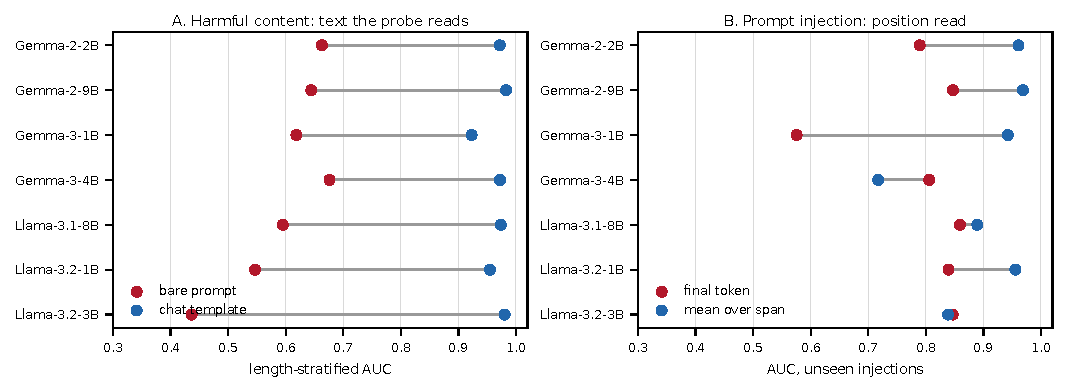
\includegraphics[width=\textwidth]{figures/fig_extraction}
\caption{The extraction convention, not the probe, decides the outcome. Each line joins one model's score under two
reads of the same activation, with everything else held fixed. \textbf{A}: harmful-content probes read at the final
token of the bare prompt versus of the prompt in the model's own chat template, for probes fitted with on-topic
negatives; length-stratified AUC rises by $+0.296$ to $+0.544$, to $0.923$--$0.983$, on all seven models. The probes
as shipped, fitted on off-topic negatives, do not share the gain: three of them regress under the templated read
(Table~\ref{tab:extraction_convention}). \textbf{B}: prompt-injection probes read at the final token versus averaged
over the tool-response span, on the grouped split in which no injection string in the test half was seen in training;
the four models on which the mean read clears the pre-registered $0.90$ pass threshold move from $0.58$--$0.85$ to
$0.94$--$0.97$, three never reach the pass band, and Gemma-3-4B is worse at the point estimate. Neither change touches
the probe or its training data.}
\label{fig:extraction}
\end{figure*}

\subsection{Template mode: reading the prompt as the model will see it}
\label{sec:template}

An instruction-tuned model never sees a bare user prompt in deployment. It sees that prompt wrapped in a chat
template that marks the turn boundary and cues the model that a response is expected. A probe can be read either way,
and the choice is rarely stated.

Table~\ref{tab:extraction_convention} holds everything else fixed---the same $300$ harmful prompts, the same $350$
benign prompts, the same layer, the same tensor, the same threshold rule---and varies only whether the final-token
activation is taken from the bare prompt or from the templated one. Three probes are shown per model: the shipped
probe as distributed, a probe trained on on-topic benign twins, and a probe trained on the off-topic negatives the
shipped probes were originally fitted with.

% GENERATED by paper/tools/gen_tables.py -- do not edit by hand.
% sources: results/gates/extraction_convention.json
\begin{table*}[!t]
\caption{Extraction convention: the same probes, prompts, layers and feature, read at the final token of the
bare prompt versus of the prompt in the model's own chat template. AUC$^{*}$ is length-stratified. JBB FPR@m is
the JailbreakBench-benign false-positive rate at the threshold whose XSTest FPR matches the shipped probe's, so
the FPR columns are comparable across probes rather than reflecting a threshold shift. Training negatives:
on-topic twins versus the off-topic set the shipped probes were trained on.}
\label{tab:extraction_convention}
\centering
\setlength{\tabcolsep}{3.5pt}
\footnotesize
\begin{tabular}{llccccccc}
\toprule
& Negatives & AUC$^{*}$ raw & AUC$^{*}$ tmpl & $\Delta$ & AUC vs JBB raw & AUC vs JBB tmpl & FPR@m raw & FPR@m tmpl \\
\midrule
Gemma-2-2B & shipped & 0.754 & 0.875 & +0.121 & 0.485 & 0.717 & 0.80 & 0.04 \\
 & on-topic & 0.663 & 0.972 & +0.309 & 0.825 & 0.909 & 0.00 & 0.00 \\
 & off-topic & 0.828 & 0.979 & +0.152 & 0.690 & 0.910 & 0.67 & 0.00 \\
\addlinespace
Gemma-2-9B & shipped & 0.841 & 0.982 & +0.142 & 0.640 & 0.937 & 0.76 & 0.05 \\
 & on-topic & 0.645 & 0.983 & +0.338 & 0.800 & 0.906 & 0.03 & 0.07 \\
 & off-topic & 0.827 & 0.982 & +0.155 & 0.824 & 0.888 & 0.43 & 0.10 \\
\addlinespace
Gemma-3-1B & shipped & 0.689 & 0.706 & +0.017 & 0.539 & 0.719 & 0.89 & 0.00 \\
 & on-topic & 0.619 & 0.923 & +0.304 & 0.789 & 0.865 & 0.05 & 0.01 \\
 & off-topic & 0.637 & 0.935 & +0.298 & 0.600 & 0.866 & 0.68 & 0.04 \\
\addlinespace
Gemma-3-4B & shipped & 0.703 & 0.687 & -0.016 & 0.578 & 0.613 & 0.29 & 0.02 \\
 & on-topic & 0.676 & 0.972 & +0.296 & 0.603 & 0.868 & 0.22 & 0.00 \\
 & off-topic & 0.692 & 0.977 & +0.285 & 0.592 & 0.862 & 0.26 & 0.00 \\
\addlinespace
Llama-3.1-8B & shipped & 0.770 & 0.387 & -0.383 & 0.456 & 0.454 & 0.99 & 0.00 \\
 & on-topic & 0.595 & 0.974 & +0.379 & 0.769 & 0.933 & 0.00 & 0.02 \\
 & off-topic & 0.767 & 0.977 & +0.209 & 0.588 & 0.936 & 0.96 & 0.05 \\
\addlinespace
Llama-3.2-1B & shipped & 0.773 & 0.753 & -0.019 & 0.672 & 0.878 & 0.91 & 0.70 \\
 & on-topic & 0.547 & 0.955 & +0.408 & 0.770 & 0.878 & 0.00 & 0.75 \\
 & off-topic & 0.780 & 0.949 & +0.169 & 0.754 & 0.864 & 0.57 & 0.99 \\
\addlinespace
Llama-3.2-3B & shipped & 0.757 & 0.959 & +0.202 & 0.531 & 0.947 & 0.99 & 0.02 \\
 & on-topic & 0.437 & 0.980 & +0.544 & 0.702 & 0.928 & 0.00 & 0.05 \\
 & off-topic & 0.778 & 0.981 & +0.204 & 0.666 & 0.923 & 0.97 & 0.24 \\
\addlinespace
\bottomrule
\end{tabular}

\footnotesize Template effect (on-topic probe, AUC$^{*}$, templated $-$ raw): min $+0.296$, max $+0.544$, mean $+0.368$; positive on all 7 models. On-topic-twins effect (templated, AUC vs JBB, on-topic $-$ off-topic): min $-0.003$, max $+0.018$, mean $+0.005$.
\end{table*}

The templated read is better on every model. For the probe trained on on-topic twins, length-stratified AUC rises by
between $+0.296$ and $+0.544$, with a mean of $+0.368$, and there is no model on which it falls. Every one of those
seven differences excludes zero under a paired case bootstrap, the weakest lower bound being $+0.228$ on Gemma-3-1B
(Appendix~\ref{app:ci}, panel A), so ``positive on all seven models'' is a statement about intervals and not only
about point estimates. The effect is largest
precisely where the bare read was worst: on Llama-3.2-3B the same direction moves from $0.437$ to $0.980$.

The claim is about probes fitted with on-topic negatives, and the scope is not decorative. The shipped probes, whose
negatives are the off-topic set they were originally fitted with, do not share it: templating helps four of them but
costs Gemma-3-4B $-0.016$, Llama-3.2-1B $-0.019$ and Llama-3.1-8B $-0.383$, the last moving from $\aucstar{} = 0.770$
to $0.387$. Templating is therefore not a universal improvement to any probe one happens to hold. What
Table~\ref{tab:extraction_convention} supports is narrower: with the release recipe's training negatives replaced by
on-topic twins and everything else held fixed, reading through the chat template improves every model.

The false-positive picture moves with it, and this is the part that matters for deployment. Reported against on-topic
benign prompts at an operating point matched to each model's shipped-probe XSTest false-positive rate, the templated
read reduces the JailbreakBench false-positive rate to between $0.00$ and $0.07$ for six of seven models, against
$0.30$--$0.99$ for the shipped bare-read probes. Threshold-free, AUC against on-topic benign prompts rises from
$0.46$--$0.67$ to $0.87$--$0.93$. Table~\ref{tab:af_verdict} evaluates this against the pre-registered criteria: six
of seven models pass all three. The seventh, Llama-3.2-1B, is not evaluable on the false-positive criterion rather
than failing it, because that criterion is defined relative to the shipped probe's XSTest false-positive rate and for
this model in templated mode that rate is $0.76$, which anchors the matched operating point at a value where the
comparison is mechanically degenerate. It passes the other two criteria.

% GENERATED by paper/tools/gen_tables.py -- do not edit by hand.
% sources: results/gates/b1/*.json
\begin{table}[!t]
\caption{AF criteria on the chat-templated read (pre-registered thresholds: length-stratified AUC $\geq 0.80$;
JailbreakBench FPR at the matched-XSTest operating point $\leq 0.30$; AUC vs JailbreakBench $\geq 0.70$).}
\label{tab:af_verdict}
\centering
\setlength{\tabcolsep}{3.5pt}
\footnotesize
\begin{tabular}{lcccc}
\toprule
Model & AUC$^{*}$ & JBB FPR@m & AUC vs JBB & Verdict \\
\midrule
Gemma-2-2B & 0.972 & 0.00 & 0.909 & pass \\
Gemma-2-9B & 0.983 & 0.07 & 0.906 & pass \\
Gemma-3-1B & 0.923 & 0.01 & 0.865 & pass \\
Gemma-3-4B & 0.972 & 0.00 & 0.868 & pass \\
Llama-3.1-8B & 0.974 & 0.02 & 0.933 & pass \\
Llama-3.2-1B & 0.955 & 0.75$^{\dagger}$ & 0.878 & n/e \\
Llama-3.2-3B & 0.980 & 0.05 & 0.928 & pass \\
\bottomrule
\end{tabular}

\footnotesize $^{\dagger}$Not evaluable: the matched operating point is anchored at this model's shipped-probe
XSTest FPR of 0.76 in templated mode, so the comparison is mechanically degenerate. Criteria 1 and 3 pass.
\end{table}

Table~\ref{tab:af_lexical} confirms the result is not a lexical artifact. The strongest cheap text baseline we could
construct reaches $\aucstar{} = 0.710$ overall and $0.637$ against on-topic benign prompts; the templated probe beats
it by between $+0.213$ and $+0.272$. The same table carries the warning that motivates the length control: the
strongest \emph{unstratified} feature is character length, at $0.903$.

% GENERATED by paper/tools/gen_tables.py -- do not edit by hand.
% sources: results/gates/lexical_baselines.json
\begin{table}[!t]
\caption{Lexical baselines for harmful-content detection: cheap text features scored on the same
$300$ HarmBench prompts against the same benign sets, with no model and no activations. The
length-stratified columns are the ones comparable with probe numbers.}
\label{tab:af_lexical}
\centering
\setlength{\tabcolsep}{3.5pt}
\footnotesize
\begin{tabular}{lcccc}
\toprule
Feature & AUC & AUC$^{*}$ & vs JBB & vs JBB$^{*}$ \\
\midrule
imperative stem & 0.683 & 0.710 & 0.362 & 0.517 \\
``how to'' pattern & 0.556 & 0.606 & 0.575 & 0.607 \\
harm lexicon (count) & 0.667 & 0.590 & 0.664 & 0.595 \\
harm lexicon (any) & 0.654 & 0.584 & 0.647 & 0.589 \\
character length & 0.903 & 0.578 & 0.768 & 0.552 \\
harm lexicon $+$ ``how to'' & 0.681 & 0.632 & 0.686 & 0.637 \\
\bottomrule
\end{tabular}

\footnotesize Strongest length-stratified baseline: imperative stem at $0.710$. Note that the strongest \emph{unstratified} feature is character
length itself, at $0.903$, which is why every AUC in this
paper is reported length-stratified.
\end{table}

\subsection{Read position: where in a long input the signal lives}
\label{sec:read}

Harmful-content probing reads a short prompt, so the final token is a reasonable place to look. Agent-injection
detection reads a scaffold in which the injected instruction sits inside a tool response, and there the final token
is the wrong place by construction: across the $1{,}054$ cases the injection ends at a median $85\,\%$ of the
tool-response span and never at its end, so a final-token read is separated from the signal by the tail of the tool
output and the turn boundary.

We compare four reads at the same layer. \emph{final} is the final prompt token. \emph{mean} averages the activation
over the tool-response span. \emph{maxpos} takes the maximum projection over positions in that span. \emph{oracle} is
read at the token where the injected instruction ends; it uses label knowledge, is never deployable, and is included
as a diagnostic upper bound---if even the oracle is weak, the limitation is in the representation rather than in the
choice of position. For benign cases, which have no injection, the oracle position is drawn from the empirical
distribution of injection-end positions in the training half, so that read position itself carries no label
information.

% GENERATED by paper/tools/gen_tables.py -- do not edit by hand.
% sources: results/gates/b2/*.json, results/gates/b2_grouped/*.json, results/gates/validity_checks.json
\begin{table*}[!t]
\caption{Prompt-injection detection by read position, on the held-out half of real InjecAgent. Left block:
the pre-registered per-case split, in which all $62$ injection strings appear in both halves. Right block: the
grouped split, in which whole injection strings are assigned to one side, so no injection in the test half was
seen in training. \emph{mean} pools over the tool-response span; mean\textsubscript{all} pools over every
prompt token and is the whole-input baseline of prior work. \emph{oracle} is handed the injection's end
position and is a diagnostic bound, never deployable. The grouped test half holds $493$ injected cases against only $59$ benign ones, drawn from $62$ distinct injection strings: grouping removes the leakage, it does not create a large sample of injection types, and the intervals in Appendix~\ref{app:ci} are correspondingly wide. Quote these AUCs with their intervals.}
\label{tab:aag_designs}
\centering
\setlength{\tabcolsep}{3.0pt}
\footnotesize
\begin{tabular}{lccccccccccc}
\toprule
& \multicolumn{5}{c}{Injections seen in training} & \multicolumn{5}{c}{Injections unseen} & \\
\cmidrule(lr){2-6}\cmidrule(lr){7-11}
Model & final & mean & mean\textsubscript{all} & maxpos & oracle & final & mean & mean\textsubscript{all} & maxpos & oracle & oracle$-$best \\
\midrule
Gemma-2-2B & 0.774 & 0.964 & 0.936 & 0.951 & 0.992 & 0.789 & 0.961 & 0.937 & 0.944 & 0.978 & +0.028 \\
Gemma-2-9B & 0.849 & 0.970 & 0.921 & 0.975 & 0.997 & 0.847 & 0.969 & 0.927 & 0.963 & 0.990 & +0.022 \\
Gemma-3-1B & 0.546 & 0.845 & 0.782 & 0.824 & 0.796 & 0.576 & 0.943 & 0.849 & 0.919 & 0.865 & -0.049 \\
Gemma-3-4B & 0.796 & 0.758 & 0.783 & 0.635 & 0.774 & 0.806 & 0.717 & 0.762 & 0.616 & 0.751 & -0.022 \\
Llama-3.1-8B & 0.853 & 0.858 & 0.784 & 0.822 & 0.987 & 0.859 & 0.889 & 0.815 & 0.825 & 0.963 & +0.129 \\
Llama-3.2-1B & 0.828 & 0.949 & 0.882 & 0.931 & 0.994 & 0.839 & 0.956 & 0.906 & 0.931 & 0.982 & +0.045 \\
Llama-3.2-3B & 0.840 & 0.818 & 0.741 & 0.747 & 0.987 & 0.847 & 0.839 & 0.763 & 0.770 & 0.961 & +0.148 \\
\bottomrule
\end{tabular}

\footnotesize Mean AUC change when injection strings are unseen: final $-0.011$, mean $-0.016$, maxpos $-0.012$, oracle $+0.005$. The result is generalisation to unseen injections, not recognition of memorised strings. Span localisation (mean $-$ mean\textsubscript{all}, unseen split): $-0.044$ to $+0.093$; positive on 6 of 7 models (intervals in Appendix~\ref{app:ci}).
\end{table*}

Averaging over the tool-response span recovers most of what the final-token read misses. On the four models on which
the mean read clears the pass threshold of $0.90$ that was pre-registered before any activation was extracted
(Section~\ref{sec:prereg}), mean-over-tool-response reading reaches $0.94$--$0.97$ against $0.58$--$0.85$ for the final-token
read trained on identical data; on those four the paired difference excludes zero, with a smallest lower bound of
$+0.067$ (Appendix~\ref{app:ci}, panel B). On the other three it does not: the interval crosses zero on Llama-3.1-8B
($+0.030$, $[-0.022, +0.082]$), on Llama-3.2-3B ($-0.008$, $[-0.062, +0.047]$) and on Gemma-3-4B, where the mean read
is worse at the point estimate ($-0.089$, $[-0.198, +0.026]$). Both figures are quoted from the grouped split, and the
full seven-model picture is in Table~\ref{tab:aag_designs} rather than summarised away.

Localisation, not pooling as such, is what the span read adds. Prior work already compares mean pooling with
last-token reads (Section~\ref{sec:related}), so Table~\ref{tab:aag_designs} carries the whole-prompt mean,
mean\textsubscript{all}, as the baseline that claim is defined against; the comparison was pre-registered with its
threshold before the run (Section~\ref{sec:prereg}). On the four passing models the tool-response mean exceeds the
whole-prompt mean by $+0.023$ to $+0.093$, every paired interval excluding zero, and by $+0.074$ and $+0.076$ on
Llama-3.1-8B and Llama-3.2-3B; only on Gemma-3-4B, where no read works, is the whole-prompt mean ahead ($-0.044$,
$[-0.106, +0.011]$). The honest reading cuts both ways: pooling over the whole input already clears the pass threshold
on three of the four models (Gemma-3-1B is the exception, at $0.849$), so most of the repair is pooling at all, and
localising the pool to the span where the threat sits is a measurable further gain rather than the whole effect. The remaining three models divide in a way worth stating: on
Llama-3.1-8B and Llama-3.2-3B no deployable read reaches the pass band, yet the oracle reaches $0.963$ and $0.961$, so
the signal is present and it is position-finding that fails to capture it without label knowledge; on Gemma-3-4B no
read works at all, and the oracle ($0.751$) is below that model's own final-token read, so there is nothing at the
injection position for a better-placed read to find.

The right-hand block of Table~\ref{tab:aag_designs} is the result we rest on. Because the corpus crosses only $62$
injection strings with $17$ user instructions, a case-level split leaves every test-half injection string present in
training, and any number computed on it measures recognition. Assigning whole injection strings to one side removes
that: the mean AUC change across models is between $-0.016$ and $+0.005$ for every read. The improvement is
generalisation to injections never seen, not memorisation. The corpus still contains only $62$ injection strings: the
grouped split removes the leakage, it does not create a large sample of injection types. The grouped test half holds
only $59$ benign cases, which
is why the intervals in Appendix~\ref{app:ci} are wide; the per-case split, with all $120$ benign cases in play,
agrees with it to within $0.016$ and is the corroboration rather than the headline.

The oracle reaches $0.96$--$0.99$ on five models, and the gap between it and the best deployable read is $+0.02$ to
$+0.15$ on those five and negative on two. Most of the available signal is therefore already reachable without label
knowledge, which is the useful form of the result: a deployable read captures nearly what a read placed by an oracle
does. A three-layer check around each model's fixed layer moves the oracle by at most $0.09$ and does not change the
ordering of the reads; we report it as a note and do not move the headline layer, since a layer selected on the
evaluation half would not be held out.

Refusal separation shows the probe is not redundant with model behaviour here. The models refuse only $3$--$25\,\%$ of
injection prompts and follow the injected instruction in $2$--$5\,\%$ of generations, so there is little behavioural
signal for the probe to be re-detecting---in contrast to harmful-content probing, where the shipped probe's flags
largely coincide with the model's own refusals (Table~\ref{tab:af_refusal}, Section~\ref{sec:topicharm}).

\subsection{Tensor identity: which activation the probe was actually trained on}
\label{sec:tensor}

The third convention is the least visible and the easiest to get wrong. A common way to capture activations is a
forward hook on a decoder layer taking the first element of its output. In HuggingFace Transformers that element is
the post-block residual stream. In vLLM, whose Gemma-2, Llama and Qwen-2 decoder layers return
\texttt{(mlp\_branch, residual)} because the residual addition is deferred to the next layer's fused normalisation,
the same line of code captures the MLP-branch output instead. The two are different tensors, and a probe fitted
through one and evaluated through the other is not the same probe.

The return convention itself is not a discovery of ours. It is documented in the tooling community---in project
writeups on capturing activations from vLLM \cite{nnsight2026hooks}, in a vLLM issue thread on the layer return
signature \cite{vllmissue12099}, and implicitly in the existence of dedicated inspection libraries that exist partly
to paper over it \cite{vllmlens}. What has not been quantified is the silent research consequence, and that is our
contribution here.

We encountered it by scoring an identical probe on identical prompts through two independent implementations and
finding a correlation of only $0.74$ where reimplementation noise should have given essentially $1.0$.
Table~\ref{tab:tensor_identity} resolves it: read as the MLP-branch output, the same probe reproduces the original
scores at $r = 0.9998$.

% GENERATED by paper/tools/gen_tables.py -- do not edit by hand.
% sources: results/phase2/p2_summary.json, results/phase2/p2_summary_mlp.json
\begin{table}[!t]
\caption{Tensor identity. A vLLM decoder layer returns \texttt{(mlp\_branch, residual)}, so a forward hook
taking \texttt{output[0]} captures the MLP-branch output, not the residual stream. Scoring the same probe on
the same prompts through an independent HuggingFace path identifies which tensor the shipped probes live in.}
\label{tab:tensor_identity}
\centering
\begin{tabular}{lcc}
\toprule
Feature read & Pearson $r$ & mean $|\Delta|$ \\
\midrule
post-block residual stream & 0.7423 & 0.0273 \\
MLP-branch output & 0.9998 & 0.0004 \\
\bottomrule
\end{tabular}

\footnotesize $n=6200$ prompts. The probes live in the MLP-branch space; every number in this
paper is computed there.
\end{table}

The failure mode is the dangerous kind, because nothing breaks. Training and evaluation used the same hook, so results
obtained this way remain internally valid and look entirely plausible; only their description is wrong, and a reader
has no way to tell. A reimplementation that agrees with the original to two decimal places may still be reading a
different tensor, and at $r = 0.74$ the disagreement is large enough to change conclusions while small enough to be
mistaken for numerical noise. ``Layer $\ell$ activation'' is therefore underspecified as a description of a probe.

The structural remedy is an interface that makes the captured tensor explicit rather than incidental to a hook's
position in a call stack; an RFC we co-authored proposes one for vLLM \cite{vllmrfc36998}. Every number in this paper is computed in
the MLP-branch space, which is where the probes under study live.

\subsection{Scope of the templating claim}
\label{sec:scope}

The claim in Section~\ref{sec:template} is made for harmful-content probing only.

``Templated'' is not one operation. For a short user prompt it wraps the text in a user turn, which is exactly what
the model sees at deployment; the templated read is the ecologically valid one and the bare read is the artifact. For
an agent scaffold it wraps an entire multi-turn transcript inside a single user turn, which corresponds to nothing
the model sees in use. For a policy-compliance case it wraps a model \emph{response} as though the model had received
it as input, which is stranger still.

We therefore report the other two tasks in both modes as observations and draw no hypothesis test from them.
Table~\ref{tab:aag_modes} gives the agent-scaffold comparison: templating helps the final-token read on four models
by $+0.04$ to $+0.15$, is neutral on two, and hurts one by $-0.14$, while the mean-span and oracle reads barely move.
That is a different pattern from the uniform, large improvement in Table~\ref{tab:extraction_convention}, and it is
consistent with the two operations being different rather than with a single effect of ``using the chat template''.

% GENERATED by paper/tools/gen_tables.py -- do not edit by hand.
% sources: results/gates/b2/*.json, results/gates/b2_templated/*.json
\begin{table}[!t]
\caption{Agent-scaffold read, bare versus chat-templated (raw / templated). Reported as an observation, not as
a test of the harmful-content result: wrapping an entire agent transcript in a user turn is a different
operation from templating a bare user prompt.}
\label{tab:aag_modes}
\centering
\setlength{\tabcolsep}{2.0pt}
\scriptsize
\begin{tabular}{lcccc}
\toprule
Model & final & mean & mean\textsubscript{all} & oracle \\
\midrule
Gemma-2-2B & 0.774 / 0.880 & 0.964 / 0.959 & 0.936 / 0.932 & 0.992 / 0.993 \\
Gemma-2-9B & 0.849 / 0.891 & 0.970 / 0.954 & 0.921 / 0.902 & 0.997 / 0.999 \\
Gemma-3-1B & 0.546 / 0.692 & 0.845 / 0.913 & 0.782 / 0.869 & 0.796 / 0.810 \\
Gemma-3-4B & 0.796 / 0.661 & 0.758 / 0.738 & 0.783 / 0.749 & 0.774 / 0.711 \\
Llama-3.1-8B & 0.853 / 0.849 & 0.858 / 0.848 & 0.784 / 0.775 & 0.987 / 0.994 \\
Llama-3.2-1B & 0.828 / 0.886 & 0.949 / 0.958 & 0.882 / 0.873 & 0.994 / 0.991 \\
Llama-3.2-3B & 0.840 / 0.841 & 0.818 / 0.809 & 0.741 / 0.753 & 0.987 / 0.990 \\
\bottomrule
\end{tabular}
\end{table}

The general form of the recommendation is not ``apply the chat template''. It is that the extraction convention is a
free parameter which current practice leaves unreported, that its effect on these tasks is larger than the effects
papers do report, and that a probe result is uninterpretable without it. Text form, token position, and tensor
identity should be stated as routinely as the layer index.

% Section 6 -- What minimal-data probes learn.
% 6.3 is the author's draft of 2026-09-05. Five figures in it conflicted with the committed results; all five were
% corrected to the results and the corrections were approved by the author on 2026-09-05, so the \disc flags are
% cleared. The refit passage was then rewritten by the author to state affirmatively that no evaluation data touched
% the probes -- a stronger fact than the original wording, and the one the corrected method actually supports.
\section{What Minimal-Data Probes Learn}
\label{sec:learn}

Section~\ref{sec:extraction} showed that where a probe is read changes what it appears to know. This section asks the
complementary question: with the extraction convention held fixed, what have these probes actually learned? The answer
differs by task, and in one case the more interesting finding is that the question cannot be answered with the
instruments available.

\subsection{Topic, not harm}
\label{sec:topicharm}

The harmful-content probes separate topic from not-topic rather than harmful from benign, and the two benign sets of
Section~\ref{sec:data} make this legible. Read at the final token of bare text, the shipped probes reach AUC
$0.90$--$1.00$ against XSTest---benign prompts that merely sound alarming---and only $0.46$--$0.67$ against
JailbreakBench benign prompts, which share their subject matter with harmful requests. The false-positive rates say
the same thing more bluntly: $0$--$17\,\%$ on XSTest against $30$--$94\,\%$ on the on-topic set. A detector that fires
on nine in ten benign requests about the same subject is not detecting harm.

This is what makes the pooled benign set a reporting hazard rather than a convenience. Pooling XSTest and
JailbreakBench yields an aggregate AUC of $0.81$--$0.91$, which reads as a working detector and conceals that
essentially all of its errors fall on one half of the benign data. It also explains the system-level result of
Section~\ref{sec:guard}: all $94$ of the probe pipeline's false positives are on-topic benign prompts.

Chat-templated reading substantially repairs this (Table~\ref{tab:extraction_convention}), which is the finding of
Section~\ref{sec:template}. What it does not do is make the probe a harm detector by construction, and the lexical
baselines of Table~\ref{tab:af_lexical} bound how much credit is due: the best cheap text feature reaches
$\aucstar{} = 0.710$, so the templated probe's margin over ``read the words'' is $+0.213$ to $+0.272$, not the whole
of its AUC.

\subsection{Paired contrastive training is not a training method}
\label{sec:paired}

A recurring proposal for minimal-data probes is to build the training set from matched pairs---each positive aligned
with a negative sharing topic, style and length---and to average the \emph{within-pair} differences, on the argument
that shared features cancel in the difference and only the safety-relevant direction survives.

The argument is sound and the method is not distinct. For $n$ complete, aligned pairs,
\begin{equation}
    \frac{1}{n}\sum_{i=1}^{n}\left(h^{+}_{i} - h^{-}_{i}\right)
    \;=\; \frac{1}{n}\sum_{i=1}^{n} h^{+}_{i} - \frac{1}{n}\sum_{i=1}^{n} h^{-}_{i},
    \label{eq:identity}
\end{equation}
which is exactly~\eqref{eq:direction}. The pairing changes the estimator not at all; the two agree to the last bit,
and our implementation asserts the equality on every model and mode rather than merely reporting it. Any difference
between a ``paired'' and an ``unpaired'' probe is therefore a difference in the training \emph{data}, and an
experiment comparing the two rules is measuring nothing.

That leaves the real question: does building the training set from on-topic pairs help? It is testable by holding the
estimator and the positive examples fixed and varying only the negatives, which is the \emph{off-topic} row of
Table~\ref{tab:extraction_convention}. Swapping $40$ on-topic benign twins for the off-topic negatives the shipped
probes were fitted with moves AUC against on-topic benign prompts by between $-0.003$ and $+0.018$---indistinguishable
from zero on every model---while the extraction change discussed above moves it by $+0.296$ to $+0.544$. The training
set was not where the leverage was.

We report this as a retirement rather than a refutation. The proposal is not wrong about pairing cancelling shared
features; it is wrong that this constitutes a distinct \emph{method}, and that part is settled by
equation~\eqref{eq:identity} rather than by measurement. What remains is the data construction, and there our claim is
the narrower empirical one: across seven models we observed no effect distinguishable from zero, against an extraction
change measured on the same probes that moved the same quantity by an order of magnitude more. We have not run an
equivalence test, so this bounds the effect as small on these models rather than establishing that it is nil.

\subsection{Policy compliance: when the evaluation cannot certify the claim}
\label{sec:apc}

Our third task asks whether a probe can distinguish giving advice from providing information---a speech-act
distinction underlying enterprise policies such as ``do not provide medical advice.'' The results here are of a
different kind from Section~\ref{sec:extraction}'s: we diagnose the failure, and then show that the natural instrument
for testing any repair is itself invalid at this text granularity.

\textbf{The minimal-data probe has no external validity.} A compliance probe trained in the standard minimal-data
recipe---fifteen authored contrastive pairs per policy, evaluated on six held-out pairs---achieves
a perfect held-out score. On an external evaluation set of $360$ labelled responses it collapses: AUC $0.14$--$0.58$
across models (Table~\ref{tab:apc_external}), and at its own calibrated threshold it flags every case---every advice
response, every information response, and all twenty refusals---in four of the six model/mode cells
(Table~\ref{tab:apc_refusal}). The perfect original score is an artifact of a six-example split; the refusal result
illustrates a measurement error we suggest is general, in which a probe's detections are never separated from the
model's own refusal behaviour, conflating ``the probe caught it'' with ``the model was never going to comply.''

% GENERATED by paper/tools/gen_tables.py -- do not edit by hand.
% sources: results/gates/b3/*.json
\begin{table*}[!t]
\caption{Policy-compliance probes on the external evaluation set, chat-templated read. \emph{shipped} is the
minimal-data probe as distributed; \emph{fresh} is the same recipe refitted on the same authored training pairs
at the same layer --- neither is fitted to the external set. Refusals are excluded from the AUC and reported
separately in Table~\ref{tab:apc_refusal}.}
\label{tab:apc_external}
\centering
\small
\begin{tabular}{llcccccc}
\toprule
Model & Probe & medical & medical$^{*}$ & financial & legal & flag adv. & flag inf. \\
\midrule
Gemma-2-9B & shipped & 0.894 & 0.893 & 0.638 & 0.617 & 1.00 & 1.00 \\
 & fresh & 0.867 & 0.889 & 0.962 & 1.000 & 0.75 & 0.15 \\
Llama-3.1-8B & shipped & 0.144 & 0.126 & 0.270 & 0.128 & 0.38 & 0.94 \\
 & fresh & 0.991 & 0.996 & 1.000 & 0.997 & 0.89 & 0.02 \\
Llama-3.2-3B & shipped & 0.408 & 0.395 & 0.598 & 0.503 & 1.00 & 1.00 \\
 & fresh & 0.986 & 0.994 & 0.978 & 1.000 & 0.95 & 0.05 \\
\bottomrule
\end{tabular}
\end{table*}
% GENERATED by paper/tools/gen_tables.py -- do not edit by hand.
% sources: results/gates/b3/*.json
\begin{table*}[!t]
\caption{The refusal band, reported separately because it is invisible inside an advice-versus-information
AUC that excludes it. A compliance probe that flags refusals fires on exactly the responses the policy is
trying to elicit. The last column is the probe's AUC separating refusals from compliant information; $0.5$
means it cannot tell them apart.}
\label{tab:apc_refusal}
\centering
\small
\begin{tabular}{lllcccc}
\toprule
Model & Mode & Probe & $n$ & flag rate & mean score & AUC vs inf. \\
\midrule
Gemma-2-9B & raw & shipped & 20 & 1.00 & +0.016 & 0.312 \\
Gemma-2-9B & raw & fresh & 20 & 0.00 & -0.208 & 0.879 \\
Gemma-2-9B & templated & shipped & 20 & 1.00 & +0.002 & 0.203 \\
Gemma-2-9B & templated & fresh & 20 & 0.60 & -0.038 & 0.167 \\
Llama-3.1-8B & raw & shipped & 20 & 0.40 & -0.005 & 0.680 \\
Llama-3.1-8B & raw & fresh & 20 & 0.00 & -0.064 & 0.716 \\
Llama-3.1-8B & templated & shipped & 20 & 0.15 & -0.014 & 0.967 \\
Llama-3.1-8B & templated & fresh & 20 & 0.70 & -0.056 & 0.057 \\
Llama-3.2-3B & raw & shipped & 20 & 1.00 & +0.006 & 0.327 \\
Llama-3.2-3B & raw & fresh & 20 & 0.00 & -0.090 & 0.916 \\
Llama-3.2-3B & templated & shipped & 20 & 1.00 & -0.004 & 0.918 \\
Llama-3.2-3B & templated & fresh & 20 & 0.50 & -0.019 & 0.102 \\
\bottomrule
\end{tabular}

\footnotesize The shipped probe flags every case in its evaluation cell --- all advice, all information and
all 20 refusals --- in 4 of the $6$ model/mode cells.
\end{table*}

\textbf{Refit probes pass---and the pass is uninterpretable.} Probes refit by the same recipe on the same fifteen
authored pairs---differing from the shipped probes only in extraction convention---reach AUC $0.99$ within-topic and
$0.98$--$1.00$ cross-topic on the external set. No evaluation data touched the probes; apparently strong evidence of
speech-act reading. But a two-token regex---the presence of second-person pronouns---achieves $0.93$--$0.95$ on the same contrasts, and $1.000$
on the hardest cells (Table~\ref{tab:apc_lexical}). The evaluation cannot distinguish a semantic classifier from a
lexical-cue detector, because in this authored set the cue and the construct coincide.

% GENERATED by paper/tools/gen_tables.py -- do not edit by hand.
% sources: results/gates/lexical_baselines.json
\begin{table*}[!t]
\caption{Lexical baselines on the policy-compliance contrasts: no model, no activations, just a count. On the
v1 evaluation set a second-person pronoun count matches or beats the probe, so that set cannot distinguish a
speech-act classifier from a cue detector. The v2 rows are the instrument built to break the cue.}
\label{tab:apc_lexical}
\centering
\small
\begin{tabular}{llccc c}
\toprule
Set & Scope & $n$ & second person & modals & length \\
\midrule
v1 medical & all bands & 220 & \textbf{0.936} & 0.885 & 0.514 \\
v1 medical & hard bands & 110 & \textbf{0.955} & 0.862 & 0.524 \\
v1 financial & all bands & 56 & \textbf{0.929} & 0.801 & 0.500 \\
v1 financial & hard bands & 28 & \textbf{0.929} & 0.768 & 0.513 \\
v1 legal & all bands & 56 & \textbf{0.946} & 0.824 & 0.518 \\
v1 legal & hard bands & 28 & \textbf{1.000} & 0.906 & 0.546 \\
v2 & all cells & 80 & \textbf{0.513} & 0.500 & 0.512 \\
v2 & incongruent cells only & 40 & \textbf{0.000} & 0.500 & 0.501 \\
\bottomrule
\end{tabular}
\end{table*}

\textbf{Controlling the cue dissolves the construct.} We attempted to build the discriminating instrument: an
evaluation set in which lexical cues and the advice/information label are decorrelated by construction. Three
successive drafts failed in three distinct ways (Table~\ref{tab:apc_construction}). The first controlled second-person
marking; a directive-modal regex then separated the classes at $0.875$. The second controlled modals; a bag-of-words
classifier separated them at $1.000$ via register---professional nouns such as \emph{clinicians} and \emph{guidelines} appearing in $28$ of $40$ information cases against $8$ of $40$
advice cases. The third drove every measured lexical cue to chance---pronouns $0.544$, modals $0.545$,
professional-register nouns $0.500$, length $0.485$, omnibus lexical classifier $0.478$ against a within-pair-swap
null of $0.435 \pm 0.084$---and in doing so dissolved the labels themselves: median within-pair similarity after stopword removal reached $0.814$,
and members of the ``advice'' class no longer carried directive force under our own pre-registered labelling rule.

% GENERATED by paper/tools/gen_tables.py -- do not edit by hand.
% sources: results/gates/validity_checks.json
\begin{table*}[!t]
\caption{Three attempts to build an evaluation set in which lexical cues and the advice/information label are
decorrelated. Each draft controlled the cue the previous one exposed, and each exposed a new one; the third
drove every measured cue to chance and dissolved the labels instead.}
\label{tab:apc_construction}
\centering
\small
\begin{tabular}{c p{0.15\textwidth} p{0.40\textwidth} p{0.26\textwidth}}
\toprule
Draft & Cue controlled & Cue exposed & Value \\
\midrule
1 & second-person pronouns & directive modals & 0.875 (regex AUC) \\
2 & directive modals & professional/third-party register (clinicians, guidelines, pharmacists: 28/40 information cases vs 8/40 advice) & 1.000 (omnibus LOO) \\
3 & register, via 40 minimal pairs & label validity dissolved & 0.814 (median within-pair content similarity after removing pronouns, articles and copulas) \\
\bottomrule
\end{tabular}

\footnotesize Draft~3 measured cues: second person $0.544$, directive modals $0.545$, professional-register nouns $0.500$, character length $0.485$; omnibus bag-of-words under leave-pair-out cross-validation $0.478$ against a within-pair-swap null of $0.435 \pm 0.084$. Label validity: median within-pair content similarity $0.814$, with 10 of $40$ pairs above $0.90$.
\end{table*}

The omnibus figure needs one methodological note, developed in Section~\ref{sec:leakage}: on minimal-pair data
leave-one-out cross-validation is invalid, because a held-out item's twin sits in the training fold carrying the
opposite label and the classifier reliably anti-predicts. Measured that way draft~3 scores $0.019$---near-perfect
separation with the sign inverted---which says nothing about lexical separability. Leave-pair-out against a
within-pair-swap null is the correct procedure and is what the figures above report.

\textbf{The finding.} The three failures share one cause, which we state as a result rather than as a limitation: in
short text, directive force is substantially constituted by its lexical markers. Pronoun address, deontic modality,
and register are not confounds of the advice/information distinction at this granularity; they are much of what the
distinction consists in. It follows that short-text authored evaluations cannot certify a semantic claim for any
compliance classifier---probe, fine-tuned model, or otherwise---because any instrument that removes the cues removes
the construct.

Two practical consequences. First, for short responses, a lexical classifier may simply be an adequate compliance
control, and claims that a representation-level method outperforms one require evidence such evaluations cannot
provide. Second, certifying semantic speech-act classification requires naturally occurring multi-sentence responses,
where directive force is carried structurally across discourse---an evaluation we scope as future work rather than
attempt with an instrument we have shown cannot answer the question.

We are careful about what this does and does not say. It is not a claim that these probes cannot read speech acts. It
is the narrower and better-supported claim that no evidence we can construct at this text granularity could establish
that they do.

% Section 7 -- Obfuscation. Diagnosed only: nothing here is repaired, and no sentence may imply otherwise.
% All numbers from the Phase 2 results files via paper/tools/gen_tables.py.
\section{Obfuscation}
\label{sec:obfuscation}

A claim that recurs in the activation-probing literature is that internal representations see through surface
transformations of the input: because the model must decode an obfuscated instruction in order to act on it, its
activations should carry the decoded meaning, and a probe reading them should be robust where a text classifier is
not. The claim is attractive and, on the models studied here, false. This section reports the anatomy of that failure.
Nothing in it is repaired; unlike Sections~\ref{sec:template} and~\ref{sec:read}, this is a diagnosis with no fix.

The study uses Gemma-2-9B and the $1{,}200$-prompt AILuminate hazard set under four conditions: plain text, Base64,
ROT13, and leetspeak. The design choice that makes it informative is the control: harmful prompts are scored against
benign prompts carrying \emph{the same} encoding. Without that control, a probe that has merely learned to recognise
Base64 reports excellent detection, and this turns out to be exactly what happens in the literature's favourable
results (Section~\ref{sec:circularity}).

\subsection{The model can decode; the probe cannot read the decoding}
\label{sec:decode}

The premise is testable directly: ask the model to decode the encoded prompt and grade what comes back.

% GENERATED by paper/tools/gen_tables.py -- do not edit by hand.
% sources: results/phase2/p1_decode.json
\begin{table}[!t]
\caption{Behavioural decode test on Gemma-2-9B: can the model recover the plaintext of an encoded prompt when
asked to? Grades are exact (normalised string match), partial (similarity $\geq 0.6$ or $\geq 60\,\%$ word
cover) and fail. No reply in either condition was a refusal, so these grades measure decoding ability rather
than safety behaviour.}
\label{tab:decode}
\centering
\setlength{\tabcolsep}{3.5pt}
\footnotesize
\begin{tabular}{lcccccc}
\toprule
Encoding & $n$ & exact & partial & fail & refusals & mean similarity \\
\midrule
base64 & 20 & 6 & 14 & 0 & 0 & 0.98 \\
rot13 & 20 & 0 & 0 & 20 & 0 & 0.24 \\
\bottomrule
\end{tabular}
\end{table}

Table~\ref{tab:decode} shows the two encodings behave completely differently. Base64 is recovered in all $20$ cases,
$6$ of them verbatim, at a mean similarity of $0.98$ to the plaintext; the misses are single-word slips. ROT13 is not
recovered at all: the model produces unrelated filler, and mean similarity is $0.24$. No reply in either condition was
a refusal, so this measures decoding ability rather than safety behaviour.

This bounds where a decoded representation could be looked for. Base64 is the condition in which the model
demonstrably forms the decoding, so it is the condition in which a decoded representation could exist to be read;
ROT13 is not, because the model never forms the decoding at all. Behavioural decoding does not by itself imply that
the decoded content is linearly recoverable at any particular position --- that is the question the sweep asks. The result also breaks the symmetry that makes ``obfuscation robustness'' sound like one property: a defence
can only inherit robustness from a capability the model actually has.

\subsection{No block, mode, or probe construction separates encoded harm}
\label{sec:sweep}

We swept every decoder block from $14$ to $35$ (roughly $33\,\%$ to $85\,\%$ depth), in both template modes, with two
probe constructions---the shipped direction and a direction retrained per block and per mode---and in both activation
spaces of Section~\ref{sec:tensor}. That is $176$ scored cells per space per encoding.

% GENERATED by paper/tools/gen_tables.py -- do not edit by hand.
% sources: results/phase2/p2_summary_mlp.json, results/phase2/p2_confounds.json
\begin{table}[!t]
\caption{Obfuscation sweep on Gemma-2-9B: the best AUC over $22$ blocks for each encoding, as
raw/length-stratified. Harmful prompts are scored against benign prompts carrying \emph{the same} encoding, so
a probe that merely detects the encoding gains nothing. Encoded columns collapse under the length control;
plain and leetspeak do not.}
\label{tab:obfuscation_sweep}
\centering
\setlength{\tabcolsep}{3pt}
\footnotesize
\begin{tabular}{llcccc}
\toprule
Probe & Mode & none & base64 & rot13 & leetspeak \\
\midrule
shipped & raw & 0.71/0.63 & 0.74/0.64 & 0.68/0.76 & 0.66/0.64 \\
shipped & templated & 0.86/0.83 & 0.83/0.66 & 0.83/0.72 & 0.75/0.76 \\
retrained & raw & 0.78/0.76 & 0.65/0.55 & 0.91/0.79 & 0.76/0.72 \\
retrained & templated & 0.84/0.86 & 0.91/0.64 & 0.85/0.74 & 0.73/0.78 \\
\bottomrule
\end{tabular}
\end{table}

Figure~\ref{fig:obfuscation} shows the sweep in full for the most favourable configuration.

\begin{figure*}[!t]
\centering
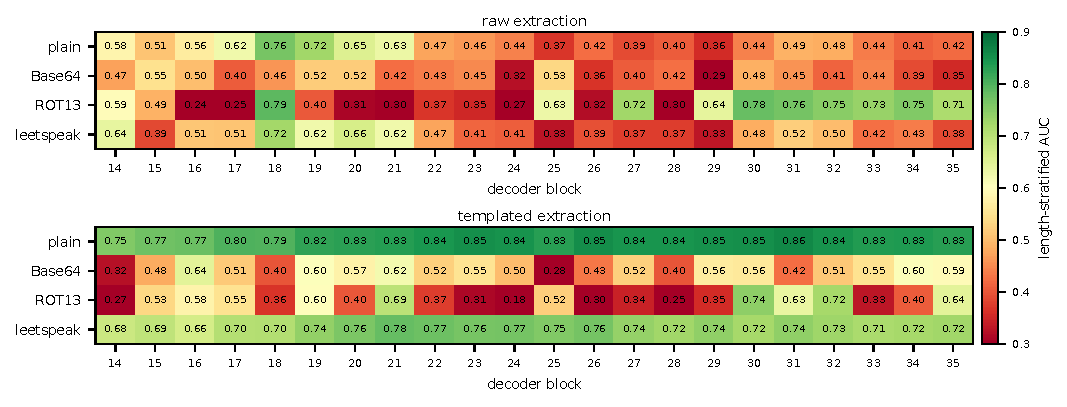
\includegraphics[width=\textwidth]{figures/fig_obfuscation}
\caption{No configuration separates encoded-harmful from encoded-benign prompts once prompt length is controlled.
Each cell is the length-stratified AUC at one decoder block, scoring harmful against benign prompts carrying the same
encoding. \textbf{The configuration shown is the best-performing one in the entire sweep}---the probe retrained per
block and per mode, read in the MLP-branch space the probes under study occupy---so what fails here is the strongest
case available, not a weak probe. Plain text and leetspeak
remain readable across the depth of the network; Base64 and ROT13 sit at or near chance everywhere, with a median of
$0.513$ over the $132$ encoded cells and a maximum of $0.787$. The uncontrolled versions of several of these cells
reach $0.85$--$0.92$, which is what length stratification removes.}
\label{fig:obfuscation}
\end{figure*}

Read the two numbers in each cell together. Several cells reach $0.85$--$0.92$ raw on Base64 and ROT13, which taken
alone would look like a positive result. In those same cells the probe score correlates with prompt length at
Spearman $\rho$ up to $+0.95$, and once length is stratified they fall to $0.49$--$0.65$. The best length-stratified
figure anywhere in the sweep is $0.73$ for Base64 and $0.79$ for ROT13, and the median across the $176$ cells is at or
below chance for both. Plain text and leetspeak lose almost nothing under the same control.

A second control settles the interpretation. If a block represented the decoded content of an encoded prompt, the
probe's score on the encoded prompt should track that same prompt's plain-text score at the same block. Across every
cell, that correlation is at most $0.36$ for Base64 and ROT13 and mostly below $0.2$, against $0.65$--$0.81$ for
leetspeak. Encoded-prompt scores carry essentially no information about what the prompt says.

Leetspeak is the exception that clarifies the rule. It leaves most characters readable, the probe treats it as noisy
plain text, and detection is nearly unchanged from plain ($46.5\,\%$ against $47.8\,\%$ at the shipped threshold). It
is not an obfuscation for this probe, and reporting it beside Base64 and ROT13 as though the three were comparable
overstates robustness considerably.

\subsection{How the favourable result is manufactured}
\label{sec:circularity}

The reason this matters is that a strong obfuscation result is easy to produce by accident.

% GENERATED by paper/tools/gen_tables.py -- do not edit by hand.
% sources: results/phase2/p3_circularity.json
\begin{table*}[!t]
\caption{Training-set circularity. Each cell reads detection / false-positive rate on \emph{equally encoded}
benign prompts / AUC. A probe whose training set contains encoded prompts reports near-perfect detection of
encoded harmful prompts while flagging just as many encoded benign ones, at below-chance AUC. Removing the
encoded prompts from training drops encoded detection to zero.}
\label{tab:circularity}
\centering
\setlength{\tabcolsep}{2pt}
\scriptsize
\begin{tabular}{llcccccccccccc}
\toprule
 & & \multicolumn{3}{c}{none} & \multicolumn{3}{c}{base64} & \multicolumn{3}{c}{rot13} & \multicolumn{3}{c}{leetspeak} \\
\cmidrule(lr){3-5} \cmidrule(lr){6-8} \cmidrule(lr){9-11} \cmidrule(lr){12-14}
Training set & Mode & det & FPR & AUC & det & FPR & AUC & det & FPR & AUC & det & FPR & AUC \\
\midrule
with encoded training prompts & raw & 0.99 & 0.72 & 0.90 & 1.00 & 1.00 & 0.29 & 1.00 & 1.00 & 0.29 & 1.00 & 1.00 & 0.77 \\
with encoded training prompts & templated & 0.77 & 0.31 & 0.82 & 1.00 & 1.00 & 0.26 & 1.00 & 1.00 & 0.04 & 0.89 & 0.73 & 0.71 \\
plain-only ablation & raw & 0.66 & 0.31 & 0.75 & 0.00 & 0.00 & 0.51 & 0.00 & 0.00 & 0.55 & 0.44 & 0.11 & 0.76 \\
plain-only ablation & templated & 0.71 & 0.19 & 0.82 & 0.00 & 0.00 & 0.53 & 0.00 & 0.00 & 0.29 & 0.74 & 0.42 & 0.72 \\
\bottomrule
\end{tabular}
\end{table*}

Table~\ref{tab:circularity} reconstructs a training recipe in which $30$ of the $81$ positive examples are themselves
encoded prompts. It reproduces the headline: essentially every Base64 and ROT13 harmful prompt is flagged. It also
flags essentially every Base64 and ROT13 \emph{benign} prompt, and the harmful-versus-benign AUC in those conditions
is $0.04$--$0.29$---below chance, because within the encoded prompts the longer ones, which are the harmful ones,
score \emph{lower}. The direction has learned ``is encoded'', not ``is harmful''. Remove the encoded examples from
training and encoded detection falls to zero.

An evaluation without an equally-encoded benign control cannot tell these two situations apart, and that control is
absent from the setups we are aware of. This is the same structure as the length confound in
Section~\ref{sec:controls}: a number that is real, reproducible, and measuring something other than the claim.

\subsection{What the probe adds over the model's own behaviour}
\label{sec:obf_refusal}

Finally, the refusal control. On plain text the probe's detections concentrate on prompts the model refuses anyway:
$81\,\%$ of refused harmful prompts are flagged against $22\,\%$ of answered ones, so the marginal value over the
model's existing behaviour is smaller than the headline detection rate suggests. Under Base64 and ROT13 the probe
detects nothing regardless of refusal---$0$ of $25$ sampled harmful prompts in both encodings---while the model itself
refuses $8$ of $25$ Base64 prompts, which it can decode, and $1$ of $25$ ROT13 prompts, which it cannot.

\subsection{What may and may not be claimed}
\label{sec:obf_claims}

Stated precisely, so that the negative result is not overread in either direction:

\begin{itemize}
\item Gemma-2-9B decodes Base64 in generation and does not decode ROT13.
\item Within the searched space --- $22$ blocks, two template modes, two probe constructions, two activation spaces,
      all at the last token --- no configuration separates Base64- or ROT13-encoded harmful prompts from equally
      encoded benign prompts once prompt length is controlled. The search did not vary read position, which
      Section~\ref{sec:read} shows can dominate everything else; that is the largest gap in this negative result.
\item Apparent successes on encoded prompts in this design are explained by prompt length, and reported successes
      elsewhere are explained by training on the encodings being tested, with no encoded benign control to expose it.
\item Leetspeak is read as noisy plain text and should not be grouped with the other two.
\end{itemize}

What this does \emph{not} establish is a general impossibility. We tested one model family at one scale, one probe
construction, and last-token reads. Section~\ref{sec:read} showed that a read position can matter more than anything
else in the setup, and we did not sweep read positions here. The honest summary is that the obfuscation-robustness
claim is unsupported on these models and that the experiments which appear to support it elsewhere have a control
missing---not that no representation of decoded content exists anywhere in any model.

% Section 8 -- Comparison to guard models. Framing rule 6: the case is cost profile, NOT accuracy.
% The guard model wins on accuracy and the section says so plainly, in its own words, in the first paragraph.
\section{Comparison to Guard Models}
\label{sec:guard}

The deployed alternative to an activation probe is a guard model: a separate classifier, itself a language model,
that reads the prompt and returns a safety verdict. Llama Guard~3 \cite{inan2023llama} is the common open reference,
and ShieldGemma \cite{zeng2024shieldgemma} and WildGuard \cite{han2024wildguard} occupy the same slot. The comparison
below runs both systems on identical inputs through their own intended interfaces.

\textbf{The guard model is more accurate, on every metric, and the probe's case is not accuracy.}
Table~\ref{tab:guard} gives the numbers: Llama Guard~3 reaches $93.5\,\%$ accuracy against the probe's $81.7\,\%$,
with a false-positive rate of $8.9\,\%$ against $26.9\,\%$ and F1 of $0.932$ against $0.822$. We state this first
because the comparison is easy to present the other way round by choosing a favourable prompt set, and because the
probe's actual advantage does not depend on winning it.

% GENERATED by paper/tools/gen_tables.py -- do not edit by hand.
% sources: results/phase1/llama_guard_comparison.json
\begin{table*}[!t]
\caption{Probe versus guard model on the same $650$ prompts ($300$ HarmBench, $250$ XSTest safe, $100$
JailbreakBench benign), each through its own intended interface. The guard model is more accurate on every
metric; the probe's case is cost, not accuracy.}
\label{tab:guard}
\centering
\small
\begin{tabular}{lccccccc}
\toprule
System & Acc.\ & TPR & FPR & Prec. & F1 & latency (ms) & p99 \\
\midrule
Probe on Llama-3.2-3B & 81.7 & 91.7 & 26.9 & 0.745 & 0.822 & 16.2 $\pm$ 1.2 & 21.1 \\
Llama Guard 3 (8B) & 93.5 & 96.3 & 8.9 & 0.903 & 0.932 & 64.7 $\pm$ 21.5 & 107.0 \\
\bottomrule
\end{tabular}

\footnotesize Mean-latency ratio $4.0\times$ on identical hardware (A100-40GB), over 3 runs. All $94$ of the probe's false positives are JailbreakBench benign prompts.
\end{table*}

The evaluation is $650$ prompts---$300$ HarmBench behaviours, $250$ XSTest safe prompts, $100$ JailbreakBench benign
prompts---with the guard model prompted through its own chat template including its hazard taxonomy, and the probe
read at its own layer and threshold. Both systems see exactly the same text.

The shape of the probe's errors is worth more than the aggregate. All $94$ of its false positives are JailbreakBench
benign prompts, and none are XSTest: the failure is entirely on on-topic benign requests, which is the topic-confound
signature of Section~\ref{sec:learn} appearing in a system-level metric. Llama Guard's false positives are spread
more evenly ($3.2\,\%$ on XSTest, $23.0\,\%$ on JailbreakBench), so it is not merely a better-calibrated version of
the same detector; it is discriminating on a partly different basis.

\subsection{Where the cost actually sits}
\label{sec:cost}

% GENERATED by paper/tools/gen_tables.py -- do not edit by hand.
% sources: results/phase1/latency/*.json
\begin{table}[!t]
\caption{Where the cost sits. The probe itself is a dot product; the forward pass it rides on is the expense,
and that pass is already being computed to serve the request. Batch size $1$, greedy, hook attached, $50$ timed
generations after $5$ warm-ups, on an A100-40GB.}
\label{tab:latency}
\centering
\setlength{\tabcolsep}{4pt}
\footnotesize
\begin{tabular}{lccc}
\toprule
Model & fwd.\ pass (ms) & p99 & probe ($\mu$s) \\
\midrule
Gemma-2-2B & 31.5 $\pm$ 0.2 & 32.1 & 1.1 \\
Gemma-2-9B & 50.0 $\pm$ 0.2 & 50.3 & 1.3 \\
Gemma-3-1B & 41.5 $\pm$ 0.2 & 42.2 & 1.0 \\
Gemma-3-4B & 61.2 $\pm$ 1.6 & 68.9 & 1.3 \\
Llama-3.1-8B & 17.7 $\pm$ 0.2 & 18.1 & 1.5 \\
Llama-3.2-1B & 10.1 $\pm$ 0.1 & 10.5 & 1.2 \\
Llama-3.2-3B & 15.9 $\pm$ 0.2 & 16.5 & 1.4 \\
\bottomrule
\end{tabular}
\end{table}

The probe's case is the cost profile, and Table~\ref{tab:latency} shows why it is not the ratio in
Table~\ref{tab:guard} that matters. The probe itself is a dot product between a $3{,}584$-dimensional activation and a
direction vector: measured at $1.2$--$1.5$ microseconds, four orders of magnitude below the forward pass it rides on.
And that forward pass is not an additional cost, because it is the pass already being run to serve the request. In a
deployment that is generating a response anyway, the marginal cost of the probe is the dot product and a hook.

A guard model has a different structure of cost: it is a second model, of comparable size to the one being guarded,
run as an extra inference. Here that is $64.7$~ms mean and $107.0$~ms at the ninety-ninth percentile against the
probe path's $16.2$~ms and $21.1$~ms, a mean ratio of $4.0\times$; but the ratio is an artifact of which host model
the probe rides on, and would change with a different one. The durable statement is architectural rather than
numerical: a probe adds microseconds to an inference that is already happening, whereas a guard model adds an
inference. Memory follows the same pattern---an $8$B guard model must be resident alongside the served model, while a
direction vector is a few kilobytes.

\textbf{Hardware caveat.} These are A100-40GB numbers on a current inference stack. Earlier figures for this codebase
were collected on an L4, where the absolute latencies and the ratio both differ; the two are not comparable, and we
report only the measurements made here. Latency ratios between a probe and a guard model should be read as a property
of a particular pairing on particular hardware, not as a constant of the method.

\subsection{What the comparison supports}
\label{sec:guard_claims}

An activation probe is not a cheaper way to get guard-model accuracy, and on this evidence it is not close. What it
offers is a detector whose marginal cost is negligible on an inference that is already being performed, which makes
it a candidate for a first-stage filter or an always-on monitor rather than a replacement for a guard model. Whether
that is worth $12$ accuracy points, and a false-positive rate concentrated precisely on benign requests that share a
topic with harmful ones, is a deployment question rather than a research one---but it should be asked with the honest
numbers in Table~\ref{tab:guard} rather than with a comparison tuned to favour the probe.

% Section 9 -- Discussion. Author's draft of 2026-09-05, cite keys mapped to refs.bib.
% One figure corrected against the committed data and flagged: the composition of the authored benign material.
\section{Discussion}
\label{sec:discussion}

\textbf{What the minimal-data regime is, and is not.} Our results do not show that activation probes fail; two of
three tasks end with probes performing strongly on real benchmarks after one-line changes to where the activation is
read. Nor do they show the minimal-data regime matches production systems: the frontier deployments we cite train on
data at scales this regime excludes by definition, and DeepMind's report of length-shift failures at production scale
\cite{gdm2026probes} suggests convention sensitivity persists even with that data. What the results show is narrower
and, we think, more useful: in the minimal-data regime, the reported number is a joint property of the probe and of
conventions most papers relegate to implementation detail. Two studies of the same recipe can honestly report
near-perfect and near-chance performance while differing only in template mode, read position, hooked tensor, or the
composition of the benign set. Until those are reported as experimental variables, results in this literature are not
comparable across papers.

\textbf{Implications for practice.} For practitioners, the repairs are free and the checklist is short: read through
the chat template; for localized threats, pool over the relevant span rather than reading the final token; verify
which tensor the serving framework's hook returns; stratify by length; include a topic-matched benign set and a
lexical baseline; separate probe detections from the model's own refusals. For consumers of probe
results---including procurement and deployment decisions---the checklist inverts into due-diligence questions, and a
reported result that cannot answer them should be treated as unmeasured rather than favorable.

\textbf{Limitations.} The obfuscation sweep covers one $9$B model exhaustively rather than many models shallowly; the
finding may not transfer to models that decode more capably. Our benign sets, though pinned and controlled, are partly
authored; Section~\ref{sec:apc}'s own finding cautions against over-trusting authored instruments, and we apply that
caution to ourselves---$40$ of the $120$ agent benign cases are authored, including $26$ of its $36$ hard negatives,
where its positives are real benchmark cases.
Distributional detection is not adversarial robustness: obfuscated-activation attacks \cite{bailey2025obfuscated} show
latent-space monitors can be actively evaded, and nothing here addresses an adaptive attacker. Benchmarks themselves
turn over; the InjecAgent artifacts we document \cite{injecagentissue7} may be repaired, at which point our measured
numbers describe a superseded version. Finally, all probes here are linear; whether the policy-compliance
construct-validity barrier or the encoded-content result changes under non-linear probes is open, though the barrier
argument in Section~\ref{sec:apc} is classifier-independent by construction.

\textbf{Why the protocol section reports its own failures.} Three of our pre-registered designs could not answer their
own questions---a split that leaked injection strings, a comparison whose two arms were algebraically identical, and
an instrument whose validity dissolved as its confounds were controlled. We report these not as confession but as
data: pre-registration's value was not that our designs were right, but that their failures were detectable,
attributable, and correctable in the open. An evaluation regime in which errors that inflate results are as
discoverable as errors that deflate them is the substantive proposal of this paper; the specific conventions are its
current, and certainly incomplete, instantiation.

% Section 10 -- Conclusion. Author's draft of 2026-09-05. The closing sentence is the thesis sentence and must remain
% identical to the one in the abstract and the introduction; tools/check_refs.py counts its occurrences.
\section{Conclusion}
\label{sec:conclusion}

We evaluated minimal-data activation probes for LLM safety across seven models and three tasks under a pre-registered
protocol, and found that reported outcomes are dominated by extraction convention and evaluation design. Two
conventions repair apparent failures without changing probe or training data: reading prompts through the model's chat
template, and pooling activations over the threat-bearing span rather than the final token. Rigorous evaluation equally
retires claims weaker evaluation supports: an estimator identical to its baseline, obfuscation robustness manufactured
by training on encodings, and a compliance task whose short-text evaluations cannot certify semantic claims for any
classifier. Two directions follow directly: an adversarial evaluation of span-pooled injection probes, since
distributional detection is not robustness; and a discourse-level compliance evaluation on naturally occurring
multi-sentence responses, the instrument our construct-validity finding shows is required. Minimal-data activation
probes can work; whether they do is decided by conventions most papers never report.

% Appendix -- confidence intervals. Every panel is a case bootstrap computed by paper/tools/gen_stats.py from committed
% per-case scores; panel B was analytic until the 2026-09-11 re-run of Arm 2 (GATES.md Amendment 7b).
\appendices
\section{Confidence Intervals on the Headline Effects}
\label{app:ci}

Table~\ref{tab:confidence} reports a $95\,\%$ interval for each of the effects the paper rests on. Every one is a
nonparametric case bootstrap over the committed per-case scores: $2{,}000$ resamples at a recorded seed, percentile
method, and the same length-stratified or plain AUC function that produced the committed point estimate, which the
tool reproduces exactly before resampling anything and aborts if it cannot.

Every difference between two reads of the same cases is resampled \emph{paired}: one draw of case indices is applied
to both arms and the difference is taken within the draw, so the positive correlation between the arms is carried in
the interval rather than assumed away. Panel B reports two such differences. The first, mean minus final, is the
repair of Section~\ref{sec:read}; the second, mean minus mean\textsubscript{all}, is the pre-registered test of
Section~\ref{sec:prereg} that the repair comes from localising the read to the tool-response span and not from
pooling as such. Resampling is stratified by class, so every resample keeps the $525$ / $59$ composition of the grouped
test half; the small benign half is why these intervals are the widest in the table.

Panel C is conditional on a selection. Each final-token row is the largest length-stratified AUC anywhere in the
sweep for that encoding---across both activation spaces, both probe constructions, both template modes and all $22$
blocks---and the pooled row is the largest Base64 cell across both spaces, both constructions, both modes, both pooled
reads and all $22$ blocks, so each interval describes the best case available to the claim of
Section~\ref{sec:obfuscation} rather than a typical cell. The median column gives the population the maximum was
drawn from, and it is the more representative number.

% GENERATED by paper/tools/gen_tables.py -- do not edit by hand.
% sources: results/gates/b1/*.json, results/gates/b2_grouped/*.json, results/gates/scores/b2_grouped_*_test_scores.json, results/phase2/p2_scores_mlp.npz, results/phase2/p2_scores.npz, results/phase2/p2_confounds.json, results/phase2/p2_summary_mlp.json, results/phase2/p2d_summary.json, results/phase2/p2d_summary_mlp.json, results/phase2/p2d_scores.npz, results/phase2/p2d_scores_mlp.npz
\begin{table*}[!t]
\caption{Ninety-five per cent confidence intervals on the three headline effects: nonparametric case
bootstraps, $2000$ resamples, seed $20260910$, percentile intervals. Every difference between two reads of the
same cases is resampled \emph{paired}: one draw of case indices is applied to both arms and the difference
taken within the draw. Panel B is computed from the per-case scores committed with the 2026-09-11 re-run of
Table~\ref{tab:aag_designs}.}
\label{tab:confidence}
\centering
\setlength{\tabcolsep}{0.8pt}
\scriptsize
\begin{tabular}{lcccccccc}
\toprule
\multicolumn{9}{l}{\textbf{A. Harmful content: bare versus templated read, on-topic probe (Table~\ref{tab:extraction_convention})}} \\
Model & \aucstar{} raw & 95\,\% CI & \aucstar{} tmpl & 95\,\% CI & $\Delta$ & 95\,\% CI & & \\
\midrule
Gemma-2-2B & 0.663 & [0.597,\,0.729] & 0.972 & [0.953,\,0.984] & +0.309 & [0.239,\,0.375] & & \\
Gemma-2-9B & 0.645 & [0.587,\,0.708] & 0.983 & [0.971,\,0.992] & +0.338 & [0.275,\,0.395] & & \\
Gemma-3-1B & 0.619 & [0.557,\,0.688] & 0.923 & [0.889,\,0.950] & +0.304 & [0.228,\,0.371] & & \\
Gemma-3-4B & 0.676 & [0.618,\,0.735] & 0.972 & [0.954,\,0.986] & +0.296 & [0.232,\,0.356] & & \\
Llama-3.1-8B & 0.595 & [0.539,\,0.666] & 0.974 & [0.952,\,0.990] & +0.379 & [0.307,\,0.436] & & \\
Llama-3.2-1B & 0.547 & [0.482,\,0.618] & 0.955 & [0.929,\,0.973] & +0.408 & [0.333,\,0.472] & & \\
Llama-3.2-3B & 0.437 & [0.376,\,0.503] & 0.980 & [0.962,\,0.993] & +0.544 & [0.475,\,0.603] & & \\
\addlinespace
\multicolumn{9}{l}{\textbf{B. Prompt injection: final, mean-over-span and whole-prompt mean, grouped split (Table~\ref{tab:aag_designs})}} \\
Model & AUC final & 95\,\% CI & AUC mean & 95\,\% CI & mean$-$final & 95\,\% CI & mean$-$mean\textsubscript{all} & 95\,\% CI \\
\midrule
Gemma-2-2B & 0.789 & [0.707,\,0.864] & 0.961 & [0.937,\,0.980] & +0.172 & [0.110,\,0.239] & +0.023 & [0.008,\,0.043] \\
Gemma-2-9B & 0.847 & [0.784,\,0.904] & 0.969 & [0.949,\,0.984] & +0.121 & [0.074,\,0.173] & +0.042 & [0.020,\,0.068] \\
Gemma-3-1B & 0.576 & [0.503,\,0.648] & 0.943 & [0.906,\,0.971] & +0.367 & [0.285,\,0.447] & +0.093 & [0.046,\,0.145] \\
Gemma-3-4B & 0.806 & [0.733,\,0.872] & 0.717 & [0.637,\,0.797] & -0.089 & [-0.198,\,0.026] & -0.044 & [-0.106,\,0.011] \\
Llama-3.1-8B & 0.859 & [0.805,\,0.907] & 0.889 & [0.843,\,0.929] & +0.030 & [-0.022,\,0.082] & +0.074 & [0.048,\,0.105] \\
Llama-3.2-1B & 0.839 & [0.777,\,0.899] & 0.956 & [0.931,\,0.976] & +0.116 & [0.067,\,0.169] & +0.050 & [0.029,\,0.071] \\
Llama-3.2-3B & 0.847 & [0.786,\,0.900] & 0.839 & [0.772,\,0.898] & -0.008 & [-0.062,\,0.047] & +0.076 & [0.049,\,0.106] \\
\addlinespace
\multicolumn{9}{l}{\textbf{C. Obfuscation: the best length-stratified cell anywhere in the sweep, per encoding (Tables~\ref{tab:obfuscation_sweep} and~\ref{tab:obfuscation_pooled})}} \\
Encoding & read & space, probe, mode & block & \aucstar{} & 95\,\% CI & median over cells & & \\
\midrule
plain & final & MLP-branch, retrained, templated & 31 & 0.860 & [0.827,\,0.891] & 0.523 & & \\
Base64 & final & residual, shipped, templated & 26 & 0.728 & [0.681,\,0.770] & 0.482 & & \\
ROT13 & final & MLP-branch, retrained, raw & 18 & 0.787 & [0.744,\,0.836] & 0.399 & & \\
leetspeak & final & residual, retrained, templated & 21 & 0.783 & [0.740,\,0.821] & 0.511 & & \\
Base64 & prompt mean & residual, retrained, raw & 19 & 0.746 & [0.700,\,0.790] & 0.598 & $\rho=+0.25$ & \\
\bottomrule
\end{tabular}

\footnotesize Panel A: every template difference excludes zero; the weakest lower bound is $+0.228$ (Gemma-3-1B). Panel B: on the 4 models whose mean read clears the pre-registered $0.90$ pass threshold the difference from the final-token read excludes zero, weakest lower bound $+0.067$; it crosses zero on Gemma-3-4B, Llama-3.1-8B, Llama-3.2-3B. The second difference, mean $-$ mean\textsubscript{all}, is what localising the read to the tool-response span adds over pooling the whole prompt: it excludes zero on 4 of those 4 models (Gemma-2-2B, Gemma-2-9B, Gemma-3-1B, Llama-3.2-1B; weakest lower bound $+0.008$). The intervals in this panel are wide because the grouped test half holds only $59$ benign cases (Section~\ref{sec:data}). Panel C: each final-token row is the maximum over $176$ cells and the pooled row over $352$, so the intervals are conditional on that selection; the median column is the population the maximum was drawn from. The best Base64 and ROT13 final-token cell does exceed chance (Section~\ref{sec:sweep} discusses that cell directly); the median does not. Pooled-read verdict on Base64 (Amendment 7): MLP-branch strengthened, residual strengthened.
\end{table*}

The re-run is deterministic: the resample seed is recorded in the table caption and in the machine-readable
\texttt{paper/stats/ci.json} the same tool writes, alongside every interval it reports.

% Back matter -- data availability, competing interests, acknowledgment (which carries the AI-use disclosure).
% The AI disclosure is a paragraph of the Acknowledgment, not a section of its own: IEEE's policy on
% AI-generated content requires it to be disclosed IN THE ACKNOWLEDGMENTS. Its wording is the author's,
% verbatim, and moving it did not change a word of it. Do not promote it back to a \section*.
% ORDER IS RECONSTRUCTED, NOT COPIED: neither prior IEEE Access paper on disk has any of these sections. The
% published AMS paper goes straight from its appendices to the biography and \EOD; the operator paper (Access-2026-
% 39837) has no back matter at all, which is the omission that got it returned to draft. The competing-interests
% wording is likewise reconstructed from the author's instruction, not copied from a prior paper.
\section*{Data and Code Availability}
\label{sec:avail}

All code, datasets, trained probes, pre-registered thresholds, decision log, and provenance-stamped results are
available at \url{https://github.com/glenfmessenger/probe-evaluation}. Every table in this paper is generated directly from committed results files; the generating commit is
recorded in the manuscript source. Benchmark artifacts documented in Section~\ref{sec:data} are reported upstream \cite{injecagentissue7}. The archive includes the policy-compliance instrument
drafts described in Section~\ref{sec:apc}; these are released as artifacts of the construction-failure finding and are
not valid evaluation sets. The IEEE template files are excluded per their license; the build documents how to obtain
them.

\section*{Competing Interests}

The author is employed by Google Cloud, which offers AI/ML infrastructure services. This research was conducted
independently and does not represent official Google products or policies.

\section*{Acknowledgment}

The author thanks the maintainers of the open benchmarks and models used in this study.

An AI assistant (Claude Code, Anthropic) built the evaluation harness, executed the experiments under the author's
pre-registered protocol, and drafted portions of the manuscript. The author designed the study, made all decisions and
sign-offs, verified all results, and approved the final text.


\bibliographystyle{IEEEtran}
\bibliography{refs}

% Author biography, no photograph (not required for this submission).
\begin{IEEEbiographynophoto}{Glen Messenger}
is a product management lead at Google Cloud, working on AI infrastructure security and AI safety. His research
focuses on representation engineering for LLM safety and inference security, with contributions in activation-based
model verification and inference-layer threat modelling; his work on detecting safety-training modification via
activation analysis appears in IEEE Access. His open-source work includes the Activation Model Scanner (AMS) and
k8s-aibom, a Kubernetes-native AI bill-of-materials framework. Prior to Google, he co-founded a B2B network security
startup and held senior security architecture roles in finance and government. He holds a CCIE certification and is a
named inventor on patents spanning firewall management and AI inference security.
\end{IEEEbiographynophoto}

\EOD

\end{document}
